% !TeX root = main.tex
\section{Optimization}

\subsection{Motivation}

Optimization is crucial for many solutions in pattern recognition, pattern analysis, machine learning and artificial intelligence. Practically every method in these fields requires solving an optimization problem, be it training a classifier, estimating model parameters, or selecting a subset of features. Optimization itself has many faces: discrete optimization (searching over a finite set of candidates), combinatorial optimization (a special case of discrete problems whose candidates are combinations, e.\,g.\ the travelling-salesperson problem), genetic algorithms (population-based stochastic search inspired by evolution), gradient descent (iterative improvement using first-order derivatives), unconstrained and constrained optimization (depending on whether the solution has to satisfy explicit constraints), linear programming (a linear objective under linear constraints), and convex optimization (a subclass with strong theoretical guarantees), among others.

For this reason, there is no lecture on pattern recognition without a refresher course on optimization techniques. Moreover, each researcher tends to have a favorite optimization algorithm, so it pays to know the whole toolbox.

\textbf{Notation in this Chapter} \\
This chapter follows the notation of Boyd \& Vandenberghe (\emph{Convex Optimization}).\autocite{boyd2004,nocedal1999}
{\small
\begin{itemize}
  \item $\vect x\in\real^d$: generic \textbf{optimization variable} (\textbf{not} a feature vector); $\vect y$ in the convexity definition is a second point in $\mathsf{dom}(f)$ (\textbf{not} a class label).
  \item $f:\real^d\rightarrow\real$: objective function; $\nabla f$ its gradient, $\nabla^2 f$ its \textbf{Hessian}.
  \item $\vect x^*$: optimal point (minimizer) of $f$.
  \item Superscript $(k)$: iteration index, e.\,g.\ $\vect x^{(k)}$ is the estimate in the $k$-th iteration.
  \item $t^{(k)}\in\real$: step length (step size) in the $k$-th iteration.
  \item $\Delta\vect x^{(k)}\in\real^d$: search direction in the $k$-th iteration.
  \item $\vect u\in\real^d$: candidate direction (unit vector w.\,r.\,t.\ a chosen norm $\|\cdot\|$).
  \item $\alpha,\beta$: parameters of the backtracking line search (not SVM parameters).
\end{itemize}
}

\subsection{Unconstrained Optimization}
 
 \textbf{Definition}

    A function $f: \real^d \rightarrow \real$ is \textbf{\emph{convex}} if the domain $\mathsf{dom}(f)$ of $f$ is a convex set \\
    and if $\forall \vect x, \vect y \in \mathsf{dom}(f)$, and $\theta$ with $0 \leq \theta \leq 1$, we have
    \begin{displaymath}
      f(\theta \vect x + (1-\theta) \vect y) \leq \theta f(\vect x) + (1-\theta) f(\vect y)
    \end{displaymath}
A function $f: \real^d \rightarrow \real$ is   \textbf{\emph{concave}} if $-f$ is convex.
   
 \textbf{Geometric interpretation:} The line segment between $(\vect x, f(\vect x))$ and $(\vect y, f(\vect y))$ lies above the graph of $f$. Let us assume in the following that we have to compute the minimum of a convex function
  \begin{displaymath}
    f: \real^d \rightarrow \real
  \end{displaymath}
  that is twice differentiable. The unconstrained optimization problem is just the solution of the minimization problem
  \begin{displaymath}
    \vect x^* = \argmin_{\vect x} f(\vect x)
  \end{displaymath}
  where $\vect x^*$ denotes the optimal point.  For this particular family of functions, a necessary and sufficient condition \\
  for the minimum is that the gradient vanishes:
  \begin{displaymath}
    \nabla f(\vect x^*) = \vect 0.
  \end{displaymath}
 Most methods follow an \textbf{iterative scheme}:
  \begin{eqnarray*}
    \mbox{initialization} & & \vect x ^{(0)}\\
    \mbox{iteration step} & & \vect x^{(k+1)}= g(\vect x^{(k)}) 
  \end{eqnarray*}
  where $g: \real^d\rightarrow \real^d$ is the update function. \\   

  The iterations  \textbf{terminate}, if 
  \begin{displaymath}
    \|\vect x^{(k+1)} - \vect x^{(k)}\| < \epsilon,
  \end{displaymath}
  i.\,e.\ no further significant change.
 
\subsection{Descent Methods}
 We now consider iteration schemes that produce a sequence of estimates \\
  according to the update function  
  \begin{displaymath}
    \vect x^{(k+1)} = g(\vect x^{(k)}) = \vect x^{(k)} + t^{(k)}\Delta \vect x^{(k)} .
  \end{displaymath}  
  where 
%  
  \begin{eqnarray*}
    \Delta \vect x^{(k)}\in \real ^d: & & \quad \mbox{is the   \textbf{search direction} in the $k$-th iteration}\\
    t^{(k)}\in \real:                & & \quad \mbox{denotes the   \textbf{step length} in the $k$-th iteration}
  \end{eqnarray*}  
  and where we expect 
%  
  \begin{displaymath}
    f( \vect x^{(k+1)} ) < f(\vect x^{(k)}) \quad \text{requires a descent direction, i.e. } \nabla f(\vect x^{(k)})^T \Delta \vect x^{(k)} < 0.
  \end{displaymath}  
  except ~~$ \vect x^{(k+1)}=\vect x^{(k)}=\vect x^*$.
  
\subsubsection{Taylor Approximation}
  For many problems it is always good to know the   \textbf{second order Taylor approximation}:
  \begin{displaymath}
    f(\vect x + t\cdot \Delta\vect x) 
    \approx f(\vect x) + t\cdot \nabla f(\vect x)^T \Delta \vect x +
      \frac{1}{2} t^2\cdot\Delta \vect x^T \nabla^2 f(\vect x)\Delta \vect x
  \end{displaymath}
  \begin{algorithmic}
    \STATE \textbf{Input:} function $f$, initial estimate $\vect x^{(0)}$\\
    \STATE Initialize: $k:=0$\\
    \Repeat
      \STATE Select (or compute) descent direction \\
      \STATE Line search (1-D optimization): $t^{(k)}= \argmin_{t \geq 0}f(\vect x^{(k)}+t\cdot \Delta\vect x^{(k)})$\\
      \STATE Update:
        \begin{displaymath}
          \vect x^{(k+1)} = \vect x^{(k)} + t^{(k)}\Delta \vect x^{(k)}
        \end{displaymath}
      \STATE $k:=k+1$\\
    \Until{$\|\vect x^{(k)} - \vect x^{(k-1)}\| < \epsilon$}\\
    \STATE \textbf{Output:} $\vect x^{(k)}$
  \end{algorithmic}
 
\subsection{Backtracking Line Search}

  \begin{itemize}  
    \item Multivariate optimization in its described form requires a proper line search method.
    \item Exact line search along the straight line $\{\vect x + t\Delta \vect x ~|~ t \geq 0\}$ has to solve
      \begin{displaymath}
        t^* = \argmin_{t\geq 0} f(\vect  x + t\Delta \vect x)
      \end{displaymath}
      and is rarely used.
    \item An overview of methods can be found in numerical recipes.
  \end{itemize}
  A simple choice is to halve the step until the function decreases sufficiently; this is the special case $\beta=\frac12$ of the algorithm below.\\
  The Armijo-Goldstein line search algorithm: 

  \begin{algorithmic}
    \STATE \textbf{Input:} function $f$, search direction $\Delta\vect x$\\
    \STATE Initialize: $t:=1$\\
    \STATE Select: $\alpha\in (0,0.5)$ and $\beta\in (0,1)$.\\
    \While{$f(\vect x + t\Delta \vect x) > f(\vect x) +  \alpha t \cdot \nabla f(\vect x)^T\Delta\vect x$}
      \STATE $t := \beta t$\\
    \EndWhile
    \STATE \textbf{Output:} $t$
  \end{algorithmic}
  Figure~\ref{fig:armijo} illustrates the sufficient decrease condition.

  \begin{figure}[htbp]
    \centering
    \begin{tikzpicture}
      \begin{axis}[width=9cm, height=6cm, xmin=0, xmax=1.05, ymin=-3.2, ymax=3.2, xlabel={step length $t$},
          ylabel={$f(\vect x+t\Delta\vect x)-f(\vect x)$}, tick label style={font=\scriptsize}, label style={font=\small},
          xtick={0,0.25,0.5,1}, legend style={font=\scriptsize, at={(0.5,-0.3)}, anchor=north, draw=none}, legend columns=1, legend cell align=left, clip=true]
        \addplot[name path=phi, black, very thick] coordinates {(0.0000,0.0000) (0.0088,-0.0621) (0.0176,-0.1218) (0.0265,-0.1791) (0.0353,-0.2341) (0.0441,-0.2868) (0.0529,-0.3374) (0.0618,-0.3859) (0.0706,-0.4323) (0.0794,-0.4768) (0.0882,-0.5194) (0.0971,-0.5601) (0.1059,-0.5990) (0.1147,-0.6361) (0.1235,-0.6716) (0.1324,-0.7054) (0.1412,-0.7376) (0.1500,-0.7682) (0.1588,-0.7973) (0.1676,-0.8248) (0.1765,-0.8510) (0.1853,-0.8756) (0.1941,-0.8989) (0.2029,-0.9208) (0.2118,-0.9414) (0.2206,-0.9606) (0.2294,-0.9785) (0.2382,-0.9951) (0.2471,-1.0105) (0.2559,-1.0246) (0.2647,-1.0375) (0.2735,-1.0492) (0.2824,-1.0596) (0.2912,-1.0688) (0.3000,-1.0768) (0.3088,-1.0837) (0.3176,-1.0893) (0.3265,-1.0937) (0.3353,-1.0970) (0.3441,-1.0990) (0.3529,-1.0999) (0.3618,-1.0995) (0.3706,-1.0979) (0.3794,-1.0951) (0.3882,-1.0910) (0.3971,-1.0857) (0.4059,-1.0791) (0.4147,-1.0713) (0.4235,-1.0621) (0.4324,-1.0515) (0.4412,-1.0397) (0.4500,-1.0264) (0.4588,-1.0117) (0.4676,-0.9956) (0.4765,-0.9780) (0.4853,-0.9588) (0.4941,-0.9382) (0.5029,-0.9159) (0.5118,-0.8920) (0.5206,-0.8664) (0.5294,-0.8390) (0.5382,-0.8099) (0.5471,-0.7789) (0.5559,-0.7460) (0.5647,-0.7112) (0.5735,-0.6744) (0.5824,-0.6354) (0.5912,-0.5943) (0.6000,-0.5509) (0.6088,-0.5052) (0.6176,-0.4572) (0.6265,-0.4066) (0.6353,-0.3535) (0.6441,-0.2977) (0.6529,-0.2391) (0.6618,-0.1776) (0.6706,-0.1132) (0.6794,-0.0457) (0.6882,0.0251) (0.6971,0.0992) (0.7059,0.1767) (0.7147,0.2579) (0.7235,0.3428) (0.7324,0.4316) (0.7412,0.5244) (0.7500,0.6214) (0.7588,0.7228) (0.7676,0.8288) (0.7765,0.9395) (0.7853,1.0551) (0.7941,1.1758) (0.8029,1.3018) (0.8118,1.4334) (0.8206,1.5708) (0.8294,1.7141) (0.8382,1.8637) (0.8471,2.0198) (0.8559,2.1827) (0.8647,2.3526) (0.8735,2.5298) (0.8824,2.7147) (0.8912,2.9075) (0.9000,3.1086)};
        \addlegendentry{$f(\vect x+t\Delta\vect x)-f(\vect x)$}
        \addplot[blue, dashed, domain=0:1.05] {-7.1860*x};
        \addlegendentry{$t\,\nabla f(\vect x)^T\Delta\vect x$ (tangent)}
        \addplot[red, thick, domain=0:1.05] {-2.1558*x};
        \addlegendentry{$\alpha t\,\nabla f(\vect x)^T\Delta\vect x$, $\alpha=0.3$}
        \addplot[only marks, mark=x, mark size=4pt, very thick, red] coordinates {(1,3.0) (0.5,-0.923)};
        \addplot[only marks, mark=*, mark size=2.5pt, green!50!black] coordinates {(0.25,-1.015)};
        \node[font=\scriptsize, anchor=north east, align=right] at (axis cs:0.98,2.9) {$t=1$: reject\\(value $+6.1$, off scale)};
        \node[font=\scriptsize, anchor=north west] at (axis cs:0.52,-0.923) {$t=\beta=0.5$: reject};
        \node[font=\scriptsize, anchor=north east] at (axis cs:0.25,-1.015) {$t=\beta^2$: accept};
      \end{axis}
    \end{tikzpicture}
    \caption{Backtracking (Armijo) line search along a descent direction $\Delta\vect x$. The step $t$ is accepted as soon as the function value lies below the red line $f(\vect x)+\alpha t\nabla f(\vect x)^T\Delta\vect x$, i.\,e.\ as soon as a fraction $\alpha$ of the decrease predicted by the linear approximation (blue, dashed) is actually achieved. Starting with $t=1$, the step is multiplied by $\beta$ until this \emph{sufficient decrease condition} holds. Here $t=1$ even increases $f$ (by about $6.1$, off scale) and $t=0.5$ decreases it too little, so the line search returns $t=\beta^2=0.25$.}
    \label{fig:armijo}
  \end{figure}
 
\subsection{Gradient Descent Methods}
 The most commonly used in machine learning. important to understand how this works. A natural choice of the search direction is the   \textbf{negative gradient}:
  
  \begin{displaymath}
    \Delta \vect x^{(k)} = -\nabla f(\vect x^{(k)})
  \end{displaymath}
\textbf{Rule of thumb:} The negative gradient is the steepest descent direction.

  \begin{algorithmic}
    \STATE \textbf{Input:} function $f$, initial estimate $\vect x^{(0)}$\\
    \STATE initialize: $k:=0$\\
    \Repeat
      \STATE Set descent direction: $\Delta\vect x^{(k)}=- \nabla f(\vect x^{(k)}) $\\
      \STATE Line search (1-D optimization): $t^{(k)}= \argmin_{t \geq 0}f(\vect x^{(k)}+t\cdot \Delta\vect x^{(k)})$\\
      \STATE Update:
        \begin{displaymath}
          \vect x^{(k+1)} = \vect x^{(k)} + t^{(k)}\Delta \vect x^{(k)} .
        \end{displaymath}
      \STATE $k:= k+1$\\
    \Until{$\|\vect x^{(k)} - \vect x^{(k-1)}\|_2 < \epsilon$}\\
    \STATE \textbf{Output:} $\vect x^{(k)}$\\
  \end{algorithmic}
 
\subsection{Steepest Descent Methods}

\subsubsection{Algorithm}
\textbf{(Normalized) steepest descent, what does it mean?} \\
We search for the unit vector that shows the largest decrease in the linear approximation of $f$:
\begin{displaymath}
  \Delta \vect x = \argmin_{\vect u} \{\nabla f(\vect x)^T \vect u ; \ \| \vect u\| = 1\}
\end{displaymath}
for a chosen norm $\|\cdot\|$ (e.\,g.\ $L_1$, $L_2$, $L_\infty$, or the quadratic norm $\|\cdot\|_{\mat P}$).

\textbf{Conclusions:}
  \begin{itemize}
    \item The steepest descent direction depends on the chosen norm.
    \item The negative gradient is not necessarily the best choice for the search direction.
  \end{itemize}
  Figure~\ref{fig:steepest_descent} shows the steepest descent direction for the same gradient and four different norms.

  \begin{figure}[htbp]
    \centering
    \begin{tikzpicture}[>={Stealth}]
      \begin{groupplot}[group style={group size=2 by 2, horizontal sep=1.0cm, vertical sep=1.2cm}, width=5.4cm, height=5.4cm,
          axis equal image, axis lines=middle, xmin=-1.8, xmax=1.8, ymin=-1.8, ymax=1.8, xtick=\empty, ytick=\empty,
          title style={font=\small}, clip=false]
        \nextgroupplot[title={$L_2$: $\Delta\vect x\propto-\nabla f$}]
          \addplot[blue, very thick, domain=0:360, samples=91, variable=\t] ({cos(\t)}, {sin(\t)});
          \draw[->, very thick, gray] (axis cs:0,0) -- (axis cs:0.8,0.45) node[above right, font=\scriptsize, black] {$\nabla f(\vect x)$};
          \draw[dashed, gray!70!black] (axis cs:-1.509,0.643) -- (axis cs:-0.234,-1.623);
          \draw[->, ultra thick, red!80!black] (axis cs:0,0) -- (axis cs:-0.872,-0.49) node[pos=1.0, below left, font=\scriptsize, black, fill=white, inner sep=1pt] {$\Delta\vect x$};
        \nextgroupplot[title={$L_1$: coordinate step}]
          \addplot[red, very thick] coordinates {(1,0) (0,1) (-1,0) (0,-1) (1,0)};
          \draw[->, very thick, gray] (axis cs:0,0) -- (axis cs:0.8,0.45) node[above right, font=\scriptsize, black] {$\nabla f(\vect x)$};
          \draw[dashed, gray!70!black] (axis cs:-1.637,1.133) -- (axis cs:-0.363,-1.133);
          \draw[->, ultra thick, red!80!black] (axis cs:0,0) -- (axis cs:-1,0) node[pos=1.0, below left, font=\scriptsize, black, fill=white, inner sep=1pt] {$\Delta\vect x$};
        \nextgroupplot[title={$L_\infty$: $-\sign(\nabla f)$}]
          \addplot[green!50!black, very thick] coordinates {(1,1) (-1,1) (-1,-1) (1,-1) (1,1)};
          \draw[->, very thick, gray] (axis cs:0,0) -- (axis cs:0.8,0.45) node[above right, font=\scriptsize, black] {$\nabla f(\vect x)$};
          \draw[dashed, gray!70!black] (axis cs:-1.637,0.133) -- (axis cs:-0.363,-2.133);
          \draw[->, ultra thick, red!80!black] (axis cs:0,0) -- (axis cs:-1,-1) node[pos=1.0, below left, font=\scriptsize, black, fill=white, inner sep=1pt] {$\Delta\vect x$};
        \nextgroupplot[title={$L_{\mat P}$: $\Delta\vect x\propto-\mat P^{-1}\nabla f$}]
          \addplot[violet, very thick, domain=0:360, samples=91, variable=\t] ({0.5*cos(\t)*cos(30)-1.2*sin(\t)*sin(30)}, {0.5*cos(\t)*sin(30)+1.2*sin(\t)*cos(30)});
          \draw[->, very thick, gray] (axis cs:0,0) -- (axis cs:0.8,0.45) node[above right, font=\scriptsize, black] {$\nabla f(\vect x)$};
          \draw[dashed, gray!70!black] (axis cs:-1.086,0.911) -- (axis cs:0.188,-1.355);
          \draw[->, ultra thick, red!80!black] (axis cs:0,0) -- (axis cs:-0.449,-0.222) node[pos=1.0, below left, font=\scriptsize, black, fill=white, inner sep=1pt] {$\Delta\vect x$};
      \end{groupplot}
    \end{tikzpicture}
    \caption{Normalized steepest descent direction $\Delta\vect x=\argmin_{\vect u}\{\nabla f(\vect x)^T\vect u;\ \|\vect u\|=1\}$ for the same gradient $\nabla f(\vect x)$ (gray) and four different norms. The unit ball of each norm is drawn around the current point $\vect x$ (origin). $\Delta\vect x$ (red) is the point of the ball that lies farthest in the direction of $-\nabla f$, i.\,e.\ where a line perpendicular to the gradient (dashed) touches the ball. For $L_2$ this is the negative gradient direction. For $L_1$ it is the corner on the axis of the largest gradient component (coordinate descent). For $L_\infty$ it is a corner of the square ($-\sign(\nabla f)$). For a quadratic norm it is $-\mat P^{-1}\nabla f$, rescaled to the ellipse.}
    \label{fig:steepest_descent}
  \end{figure}
  We consider now the first order Taylor approximation of $f(\vect x +\vect u)$ around the selected position $\vect x$:
  \begin{displaymath}
    f(\vect x+\vect u) \approx f(\vect x) + \nabla f(\vect x)^T \vect u.
  \end{displaymath}
  \begin{itemize}
    \item Here $ \nabla f(\vect x)^T \vect u$ is the directional derivative at $\vect x$ in direction $\vect u$.
    \item The vector $\vect u$ denotes a descent direction if the inner product with the gradient vector is negative, i.\,e.
      \begin{displaymath}
        \nabla f(\vect x)^T \vect u < 0~.
      \end{displaymath}
  \end{itemize}
 
  \begin{algorithmic}
    \STATE \textbf{Input:} function $f$, initial estimate $\vect x^{(0)}$, norm $\|.\|$\\
    \STATE initialize: $k:=0$\\
    \Repeat
      \STATE Compute highest descent direction: $\Delta \vect x ^{(k)}= \argmin_{\vect u} \{\nabla f(\vect x^{(k)})^T \vect u ; \ \| \vect u\| = 1\}$\\
      \STATE Line search (1-D optimization): $t^{(k)}= \argmin_{t \geq 0}f(\vect x^{(k)}+t\cdot \Delta\vect x^{(k)})$\\
      \STATE Update:
        \begin{displaymath}
          \vect x^{(k+1)} = \vect x^{(k)} + t^{(k)}\Delta \vect x^{(k)} .
        \end{displaymath}
      \STATE $k:=k+1$\\
    \Until{$\|\vect x^{(k)} - \vect x^{(k-1)}\| < \epsilon$}\\
    \STATE \textbf{Output:} $\vect x^{(k)}$\\
  \end{algorithmic}
 
\subsubsection{\texorpdfstring{$L_2$}{L2}-norm}
  For the $L_2$-norm the steepest descent direction is the direction of the negative gradient:
  \begin{displaymath}
    \Delta \vect x
    = \argmin_{\vect u} \{\nabla f(\vect x)^T \vect u ; \ \| \vect u\|_2 = 1\}
    = -\frac{\nabla f(\vect x)}{\|\nabla f(\vect x)\|_2}
  \end{displaymath}
  {\small (In practice the unnormalized $\Delta\vect x = -\nabla f(\vect x)$ is used; the line search adapts the step length.)}

\subsubsection{\texorpdfstring{$L_1$}{L1}-norm}

  The unit ball for the $L_1$-norm is a diamond (Figs.~\ref{fig:unitballs} and~\ref{fig:steepest_descent}).
   \begin{itemize}
    \item The steepest descent for the $L_1$-norm selects in each iteration 
      the component of $\nabla f(\vect x)$ with maximum absolute value and then 
      decreases or increases dependent on the sign of the selected component.   
    \item Let $i$ be the index of the gradient component with maximum absolute 
      value, and let $\vect e_i\in\real^d$ denote the corresponding base vector.
      The steepest descent direction is given by:
      \begin{eqnarray*}
        \Delta \vect x &=& \argmin_{\vect u} \{\nabla f(\vect x)^T \vect u ; \ \| \vect u\|_1 = 1\} \\
                      &=& -\sign\left(\frac{\partial}{\partial x_i} f(\vect x)\right)\vect e_i
      \end{eqnarray*}
        
    \item  \textbf{Note:} Steepest descent using the $L_1$-norm results in the {\em coordinate descent algorithm}.
  \end{itemize}
   
\subsubsection{\texorpdfstring{$L_\infty$}{L-infinity}-norm}

  The unit ball for the $L_\infty$-norm is a (hyper)cube (Figs.~\ref{fig:unitballs} and~\ref{fig:steepest_descent}). The steepest descent direction moves every component by the same amount against the sign of its partial derivative:
  \begin{displaymath}
    \Delta \vect x = \argmin_{\vect u} \{\nabla f(\vect x)^T \vect u ; \ \| \vect u\|_\infty = 1\}
    = -\,\sign\big(\nabla f(\vect x)\big) \quad\text{(componentwise)}.
  \end{displaymath}
  
\subsubsection{Quadratic norm \texorpdfstring{$\|\cdot\|_{\mat P}$}{quadratic norm}}

The unit ball for the quadratic norm $\|\vect u\|_{\mat P} = (\vect u^T\mat P\vect u)^{\frac{1}{2}}$, where $\mat P\in\real^{d\times d}$ is symmetric positive definite.

The \textbf{steepest descent} for the norm $\|\cdot\|_{\mat P}$ is given by:
\begin{eqnarray*}
  \Delta \vect x
    &=& \argmin_{\vect u} \{\nabla f(\vect x)^T \vect u ; \ \| \vect u\|_{\mat P} = 1\} \\   
    &=& \argmin_{\vect u} \{\nabla f(\vect x)^T \vect u ;\  (\vect u^T{\mat P}\vect u)^{\frac{1}{2}} = 1\} \\   
    &=& \argmin_{\vect u} \{\nabla f(\vect x)^T \vect u ;\ \| {\mat P}^{\frac{1}{2}} \vect u\|_2 = 1\}~.
\end{eqnarray*}

As we did in the LDA transform, we introduce a change of variables that makes the unit ball \textbf{spherical}:
\begin{displaymath}
  \vect x' = {\mat P}^{\frac{1}{2}} \vect x, \qquad \vect u' = {\mat P}^{\frac{1}{2}} \vect u \quad (\mbox{thus } \|\vect u\|_{\mat P} = \|\vect u'\|_2)
\end{displaymath}

and define the transformed objective
\begin{displaymath}
  f'(\vect x') = f({\mat P}^{-\frac{1}{2}}\vect x') = f(\vect x)~.
\end{displaymath}

Instead of $f(\vect x)$ we now minimize $f'(\vect x')$ using the $L_2$-norm and back-transform the result:
\begin{eqnarray*}
  \Delta \vect x'
    &=& \argmin_{\vect u'} \{\nabla f'(\vect x')^T \vect u' ; \ \| \vect u'\|_{2} = 1\} \\[.15cm]
    &\propto& -\nabla f'(\vect x') \\[.15cm]
    &=& -\mat P^{-\frac{1}{2}}\nabla f({\mat P}^{-\frac{1}{2}}\vect x') \\[.15cm]
    &=& - {\mat P}^{-\frac{1}{2}}\nabla f(\vect x)
\end{eqnarray*}
{\small $\propto$: equal up to a positive scale factor (the normalization), which is absorbed by the line search.}

Now we get for $\Delta \vect x$:
\begin{eqnarray*}
  \Delta \vect x
    &=& {\mat P}^{-\frac{1}{2}} \Delta \vect x' \\[.15cm]
    &\propto& {\mat P}^{-\frac{1}{2}} \left( - {\mat P}^{-\frac{1}{2}}\nabla f(\vect x) \right) \\[.15cm]
    &=& - \mat{P}^{-1} \nabla f(\vect x)~.
\end{eqnarray*}

\textbf{Conclusion:} The (unnormalized) steepest descent direction for the norm $\|\cdot\|_{\mat P}$ is
\begin{displaymath}
   \Delta \vect x = -\mat{P}^{-1} \nabla f(\vect x)~.
\end{displaymath}

\subsection{Newton's Method}
   \textbf{The idea:}
  \begin{itemize}
    \item Select a point.
    \item Compute the minimum of the second order Taylor approximation.
  \end{itemize}
 Second order Taylor approximation:
  \begin{displaymath}
    f(\vect x+\Delta \vect x) 
    \approx f(\vect x) + \nabla f(\vect x)^T \Delta \vect x + \frac{1}{2} \Delta \vect x^T (\nabla^2 f(\vect x))\Delta \vect x 
  \end{displaymath}
  Now we select $\Delta \vect x$ such that 
  \begin{displaymath}
    \nabla\{  f(\vect x) + \nabla f(\vect x)^T \Delta \vect x + \frac{1}{2}\Delta \vect x^T (\nabla^2 f(\vect x))\Delta \vect x\} 
    = 0
  \end{displaymath}
  Obviously the gradient is
  \begin{displaymath}
    \nabla f(\vect x)+ \nabla^2 f(\vect x)\Delta \vect x 
    = 0
  \end{displaymath}
  and thus
  \begin{displaymath}
    \Delta \vect x 
    = -(\nabla^2 f(\vect x))^{-1} \nabla f(\vect x)
  \end{displaymath} 
\textbf{Conclusion:} \\
  Newton's method is an $\vect x$-dependent steepest descent method regarding the quadratic norm $\|\cdot\|_{\mat P}$, where $\mat P = \nabla^2 f(\vect x)$ is the Hessian (assumed positive definite).
  Figure~\ref{fig:gd_vs_newton} compares gradient descent and Newton's method on a 2-D example.

  \begin{figure}[htbp]
    \centering
    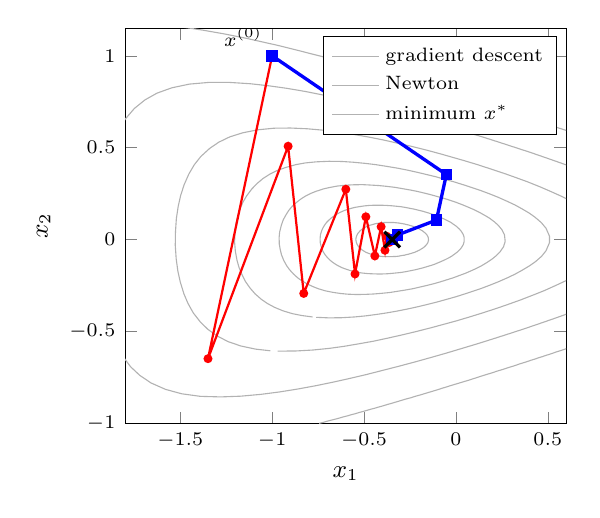
\begin{tikzpicture}
      \begin{axis}[width=8.6cm, height=6.6cm, xmin=-1.8, xmax=0.6, ymin=-1.0, ymax=1.15, axis equal image,
          xlabel={$x_1$}, ylabel={$x_2$}, tick label style={font=\scriptsize}, label style={font=\small},
          legend style={font=\scriptsize, at={(0.98,0.98)}, anchor=north east}, legend cell align=left]
\addplot[gray!60, thin] coordinates {(-0.410,-0.091) (-0.411,-0.091) (-0.420,-0.089) (-0.430,-0.088) (-0.440,-0.086) (-0.450,-0.083) (-0.450,-0.083) (-0.460,-0.080) (-0.470,-0.077) (-0.473,-0.076) (-0.480,-0.073) (-0.490,-0.069) (-0.490,-0.069) (-0.500,-0.063) (-0.503,-0.061) (-0.510,-0.057) (-0.513,-0.054) (-0.520,-0.048) (-0.522,-0.047) (-0.529,-0.039) (-0.530,-0.038) (-0.534,-0.032) (-0.538,-0.025) (-0.540,-0.020) (-0.541,-0.017) (-0.543,-0.010) (-0.544,-0.003) (-0.544,0.005) (-0.543,0.012) (-0.540,0.019) (-0.540,0.020) (-0.537,0.027) (-0.533,0.034) (-0.530,0.038) (-0.527,0.041) (-0.520,0.049) (-0.520,0.049) (-0.511,0.056) (-0.510,0.057) (-0.500,0.063) (-0.500,0.063) (-0.490,0.069) (-0.486,0.071) (-0.480,0.073) (-0.470,0.077) (-0.468,0.078) (-0.460,0.080) (-0.450,0.083) (-0.442,0.085) (-0.440,0.086) (-0.430,0.088) (-0.420,0.089) (-0.410,0.091) (-0.400,0.092) (-0.390,0.093) (-0.389,0.093) (-0.380,0.093) (-0.370,0.093) (-0.360,0.093) (-0.350,0.093) (-0.343,0.093) (-0.340,0.093) (-0.330,0.092) (-0.320,0.091) (-0.310,0.090) (-0.300,0.088) (-0.290,0.087) (-0.284,0.085) (-0.280,0.085) (-0.270,0.082) (-0.260,0.080) (-0.253,0.078) (-0.250,0.077) (-0.240,0.074) (-0.230,0.071) (-0.230,0.071) (-0.220,0.067) (-0.211,0.063) (-0.210,0.063) (-0.200,0.058) (-0.196,0.056) (-0.190,0.052) (-0.184,0.049) (-0.180,0.046) (-0.174,0.041) (-0.170,0.038) (-0.166,0.034) (-0.160,0.028) (-0.159,0.027) (-0.154,0.019) (-0.151,0.012) (-0.150,0.007) (-0.150,0.005) (-0.149,-0.003) (-0.150,-0.007) (-0.151,-0.010) (-0.153,-0.017) (-0.158,-0.025) (-0.160,-0.027) (-0.164,-0.032) (-0.170,-0.038) (-0.171,-0.039) (-0.180,-0.046) (-0.181,-0.047) (-0.190,-0.052) (-0.193,-0.054) (-0.200,-0.058) (-0.207,-0.061) (-0.210,-0.063) (-0.220,-0.067) (-0.224,-0.069) (-0.230,-0.071) (-0.240,-0.074) (-0.246,-0.076) (-0.250,-0.077) (-0.260,-0.080) (-0.270,-0.082) (-0.274,-0.083) (-0.280,-0.085) (-0.290,-0.086) (-0.300,-0.088) (-0.310,-0.090) (-0.319,-0.091) (-0.320,-0.091) (-0.330,-0.092) (-0.340,-0.092) (-0.350,-0.093) (-0.360,-0.093) (-0.370,-0.093) (-0.380,-0.093) (-0.390,-0.093) (-0.400,-0.092) (-0.410,-0.091)};
\addplot[gray!60, thin] coordinates {(-0.460,-0.186) (-0.480,-0.185) (-0.510,-0.182) (-0.530,-0.179) (-0.560,-0.172) (-0.580,-0.167) (-0.600,-0.160) (-0.620,-0.153) (-0.640,-0.143) (-0.654,-0.135) (-0.670,-0.124) (-0.684,-0.113) (-0.699,-0.098) (-0.710,-0.085) (-0.720,-0.070) (-0.728,-0.054) (-0.733,-0.039) (-0.738,-0.017) (-0.739,0.005) (-0.737,0.027) (-0.730,0.049) (-0.724,0.063) (-0.715,0.078) (-0.704,0.093) (-0.690,0.107) (-0.680,0.116) (-0.663,0.129) (-0.650,0.137) (-0.630,0.148) (-0.610,0.157) (-0.590,0.164) (-0.570,0.170) (-0.550,0.175) (-0.520,0.180) (-0.500,0.183) (-0.470,0.186) (-0.440,0.187) (-0.410,0.187) (-0.380,0.186) (-0.350,0.184) (-0.320,0.181) (-0.300,0.179) (-0.270,0.174) (-0.250,0.170) (-0.229,0.166) (-0.200,0.159) (-0.180,0.154) (-0.160,0.148) (-0.140,0.142) (-0.120,0.135) (-0.100,0.128) (-0.080,0.119) (-0.060,0.110) (-0.040,0.100) (-0.027,0.093) (-0.010,0.081) (0.004,0.071) (0.020,0.056) (0.030,0.044) (0.040,0.027) (0.045,0.012) (0.045,-0.010) (0.040,-0.027) (0.030,-0.044) (0.020,-0.056) (0.006,-0.069) (-0.010,-0.081) (-0.024,-0.091) (-0.040,-0.100) (-0.060,-0.110) (-0.080,-0.119) (-0.099,-0.127) (-0.118,-0.135) (-0.140,-0.142) (-0.160,-0.148) (-0.180,-0.154) (-0.200,-0.159) (-0.220,-0.164) (-0.250,-0.170) (-0.270,-0.174) (-0.300,-0.179) (-0.320,-0.181) (-0.350,-0.184) (-0.373,-0.186) (-0.400,-0.187) (-0.430,-0.187) (-0.460,-0.186)};
\addplot[gray!60, thin] coordinates {(-0.590,-0.297) (-0.630,-0.293) (-0.670,-0.287) (-0.710,-0.279) (-0.750,-0.267) (-0.780,-0.255) (-0.810,-0.241) (-0.840,-0.223) (-0.861,-0.208) (-0.885,-0.186) (-0.905,-0.164) (-0.921,-0.142) (-0.937,-0.113) (-0.949,-0.083) (-0.956,-0.054) (-0.961,-0.025) (-0.962,0.012) (-0.959,0.041) (-0.950,0.078) (-0.940,0.106) (-0.928,0.129) (-0.910,0.158) (-0.891,0.181) (-0.870,0.200) (-0.849,0.217) (-0.820,0.236) (-0.790,0.251) (-0.760,0.263) (-0.720,0.276) (-0.689,0.283) (-0.647,0.291) (-0.600,0.296) (-0.560,0.298) (-0.510,0.299) (-0.470,0.297) (-0.420,0.294) (-0.380,0.290) (-0.330,0.284) (-0.290,0.277) (-0.250,0.270) (-0.210,0.262) (-0.176,0.254) (-0.140,0.245) (-0.100,0.234) (-0.067,0.225) (-0.030,0.213) (0.000,0.203) (0.039,0.188) (0.070,0.175) (0.100,0.162) (0.130,0.147) (0.160,0.130) (0.185,0.115) (0.210,0.096) (0.230,0.078) (0.250,0.054) (0.264,0.027) (0.268,-0.010) (0.259,-0.039) (0.240,-0.067) (0.220,-0.087) (0.198,-0.105) (0.170,-0.124) (0.140,-0.142) (0.111,-0.157) (0.080,-0.171) (0.050,-0.184) (0.020,-0.195) (-0.015,-0.208) (-0.050,-0.219) (-0.085,-0.230) (-0.120,-0.240) (-0.160,-0.250) (-0.199,-0.259) (-0.233,-0.267) (-0.272,-0.274) (-0.316,-0.281) (-0.360,-0.288) (-0.400,-0.292) (-0.447,-0.296) (-0.490,-0.298) (-0.540,-0.299) (-0.590,-0.297)};
\addplot[gray!60, thin] coordinates {(-0.780,-0.421) (-0.840,-0.413) (-0.890,-0.403) (-0.940,-0.388) (-0.986,-0.369) (-1.027,-0.347) (-1.060,-0.324) (-1.092,-0.296) (-1.120,-0.264) (-1.144,-0.230) (-1.163,-0.193) (-1.180,-0.152) (-1.191,-0.113) (-1.200,-0.064) (-1.204,-0.017) (-1.203,0.034) (-1.198,0.078) (-1.189,0.122) (-1.175,0.166) (-1.159,0.203) (-1.138,0.239) (-1.110,0.276) (-1.082,0.305) (-1.050,0.332) (-1.011,0.357) (-0.970,0.377) (-0.924,0.393) (-0.870,0.408) (-0.820,0.417) (-0.760,0.423) (-0.690,0.426) (-0.620,0.425) (-0.560,0.421) (-0.497,0.415) (-0.438,0.408) (-0.380,0.399) (-0.320,0.389) (-0.269,0.379) (-0.210,0.366) (-0.160,0.354) (-0.110,0.342) (-0.057,0.327) (-0.007,0.313) (0.041,0.298) (0.090,0.282) (0.140,0.265) (0.188,0.247) (0.230,0.230) (0.275,0.210) (0.320,0.189) (0.360,0.167) (0.399,0.144) (0.430,0.122) (0.464,0.093) (0.490,0.062) (0.509,0.019) (0.509,-0.017) (0.490,-0.061) (0.466,-0.091) (0.433,-0.120) (0.400,-0.143) (0.360,-0.167) (0.320,-0.189) (0.280,-0.208) (0.230,-0.230) (0.190,-0.246) (0.140,-0.265) (0.092,-0.281) (0.047,-0.296) (0.000,-0.311) (-0.050,-0.325) (-0.104,-0.340) (-0.160,-0.354) (-0.210,-0.366) (-0.260,-0.377) (-0.320,-0.389) (-0.377,-0.399) (-0.430,-0.407) (-0.490,-0.415) (-0.552,-0.421) (-0.620,-0.425) (-0.690,-0.426) (-0.760,-0.423)};
\addplot[gray!60, thin] coordinates {(-1.010,-0.605) (-1.090,-0.596) (-1.170,-0.579) (-1.240,-0.555) (-1.300,-0.524) (-1.350,-0.488) (-1.390,-0.449) (-1.429,-0.399) (-1.458,-0.347) (-1.480,-0.295) (-1.500,-0.230) (-1.513,-0.171) (-1.522,-0.105) (-1.527,-0.032) (-1.526,0.041) (-1.521,0.115) (-1.511,0.181) (-1.498,0.239) (-1.479,0.298) (-1.453,0.357) (-1.423,0.408) (-1.388,0.452) (-1.340,0.496) (-1.290,0.530) (-1.230,0.559) (-1.160,0.581) (-1.080,0.597) (-0.990,0.606) (-0.900,0.607) (-0.810,0.603) (-0.720,0.595) (-0.632,0.584) (-0.550,0.571) (-0.470,0.557) (-0.390,0.541) (-0.320,0.525) (-0.240,0.507) (-0.168,0.489) (-0.090,0.468) (-0.020,0.448) (0.050,0.428) (0.120,0.407) (0.190,0.384) (0.260,0.361) (0.330,0.336) (0.393,0.313) (0.460,0.286) (0.520,0.260) (0.582,0.232) (0.640,0.202) (0.700,0.167) (0.750,0.131) (0.792,0.093) (0.825,0.041) (0.831,-0.025) (0.805,-0.076) (0.764,-0.120) (0.715,-0.157) (0.660,-0.191) (0.600,-0.223) (0.540,-0.251) (0.480,-0.278) (0.417,-0.303) (0.350,-0.329) (0.280,-0.354) (0.213,-0.377) (0.145,-0.399) (0.074,-0.421) (0.000,-0.443) (-0.070,-0.462) (-0.140,-0.481) (-0.219,-0.501) (-0.290,-0.518) (-0.370,-0.536) (-0.449,-0.553) (-0.528,-0.567) (-0.610,-0.581) (-0.690,-0.592) (-0.780,-0.601) (-0.870,-0.606) (-0.970,-0.607)};
\addplot[gray!60, thin] coordinates {(1.000,-0.238) (0.926,-0.274) (0.850,-0.308) (0.773,-0.340) (0.698,-0.369) (0.620,-0.399) (0.539,-0.428) (0.455,-0.457) (0.370,-0.486) (0.290,-0.512) (0.209,-0.538) (0.120,-0.566) (0.040,-0.590) (-0.050,-0.617) (-0.134,-0.641) (-0.220,-0.665) (-0.310,-0.689) (-0.400,-0.712) (-0.490,-0.735) (-0.580,-0.756) (-0.670,-0.776) (-0.762,-0.795) (-0.860,-0.813) (-0.960,-0.829) (-1.060,-0.842) (-1.170,-0.852) (-1.280,-0.856) (-1.390,-0.853) (-1.492,-0.839) (-1.580,-0.815) (-1.659,-0.780) (-1.720,-0.739) (-1.770,-0.692) (-1.814,-0.633) (-1.850,-0.567) (-1.876,-0.501) (-1.897,-0.428) (-1.913,-0.355) (-1.925,-0.274) (-1.933,-0.193) (-1.938,-0.105) (-1.940,-0.025) (-1.940,0.056) (-1.936,0.144) (-1.930,0.226) (-1.920,0.309) (-1.906,0.386) (-1.889,0.459) (-1.864,0.533) (-1.834,0.599) (-1.798,0.657) (-1.750,0.713) (-1.692,0.760) (-1.626,0.797) (-1.545,0.826) (-1.450,0.846) (-1.346,0.855) (-1.230,0.855) (-1.120,0.848) (-1.020,0.837) (-0.920,0.823) (-0.820,0.806) (-0.730,0.788) (-0.631,0.767) (-0.540,0.746) (-0.450,0.725) (-0.360,0.702) (-0.274,0.679) (-0.190,0.656) (-0.100,0.631) (-0.014,0.606) (0.070,0.581) (0.156,0.555) (0.240,0.528) (0.320,0.502) (0.406,0.474) (0.490,0.445) (0.570,0.417) (0.650,0.388) (0.730,0.357) (0.804,0.327) (0.880,0.295) (0.953,0.261)};
\addplot[gray!60, thin] coordinates {(1.000,-0.454) (0.980,-0.461) (0.960,-0.468) (0.940,-0.476) (0.920,-0.483) (0.900,-0.490) (0.880,-0.497) (0.860,-0.504) (0.840,-0.511) (0.820,-0.518) (0.800,-0.525) (0.780,-0.532) (0.760,-0.539) (0.740,-0.546) (0.720,-0.553) (0.699,-0.560) (0.678,-0.567) (0.656,-0.575) (0.635,-0.582) (0.613,-0.589) (0.591,-0.597) (0.570,-0.604) (0.550,-0.610) (0.530,-0.617) (0.510,-0.624) (0.490,-0.630) (0.470,-0.637) (0.450,-0.643) (0.430,-0.650) (0.410,-0.656) (0.390,-0.663) (0.368,-0.670) (0.345,-0.677) (0.323,-0.685) (0.300,-0.692) (0.280,-0.698) (0.260,-0.705) (0.240,-0.711) (0.220,-0.717) (0.200,-0.724) (0.180,-0.730) (0.160,-0.736) (0.138,-0.743) (0.114,-0.751) (0.091,-0.758) (0.070,-0.765) (0.050,-0.771) (0.030,-0.777) (0.010,-0.783) (-0.010,-0.789) (-0.030,-0.795) (-0.052,-0.802) (-0.076,-0.809) (-0.100,-0.817) (-0.120,-0.823) (-0.140,-0.829) (-0.160,-0.835) (-0.180,-0.841) (-0.200,-0.847) (-0.222,-0.853) (-0.247,-0.861) (-0.270,-0.867) (-0.290,-0.873) (-0.310,-0.879) (-0.330,-0.885) (-0.350,-0.891) (-0.372,-0.897) (-0.398,-0.905) (-0.420,-0.911) (-0.440,-0.917) (-0.460,-0.922) (-0.480,-0.928) (-0.501,-0.934) (-0.527,-0.941) (-0.550,-0.948) (-0.570,-0.953) (-0.590,-0.959) (-0.610,-0.964) (-0.634,-0.971) (-0.660,-0.978) (-0.680,-0.983) (-0.700,-0.988) (-0.720,-0.994) (-0.744,-1.000)};
\addplot[gray!60, thin] coordinates {(-2.000,1.151) (-1.960,1.160) (-1.920,1.166) (-1.878,1.171) (-1.830,1.174) (-1.780,1.176) (-1.730,1.175) (-1.680,1.173) (-1.635,1.171) (-1.590,1.167) (-1.550,1.163) (-1.500,1.157) (-1.460,1.152) (-1.420,1.146) (-1.380,1.140) (-1.340,1.133) (-1.300,1.126) (-1.260,1.119) (-1.220,1.111) (-1.180,1.103) (-1.140,1.095) (-1.100,1.086) (-1.060,1.077) (-1.020,1.068) (-0.988,1.061) (-0.950,1.052) (-0.910,1.042) (-0.870,1.032) (-0.838,1.024) (-0.800,1.014) (-0.760,1.004) (-0.724,0.995) (-0.690,0.986) (-0.650,0.975) (-0.615,0.965) (-0.580,0.956) (-0.540,0.945) (-0.508,0.936) (-0.470,0.925) (-0.430,0.914) (-0.400,0.905) (-0.360,0.894) (-0.329,0.885) (-0.290,0.873) (-0.254,0.863) (-0.220,0.853) (-0.180,0.841) (-0.150,0.832) (-0.110,0.820) (-0.080,0.811) (-0.040,0.798) (-0.010,0.789) (0.030,0.777) (0.061,0.767) (0.100,0.755) (0.132,0.745) (0.170,0.733) (0.201,0.723) (0.240,0.711) (0.271,0.701) (0.310,0.689) (0.340,0.679) (0.380,0.666) (0.410,0.656) (0.450,0.643) (0.480,0.633) (0.519,0.621) (0.550,0.610) (0.585,0.599) (0.620,0.587) (0.650,0.577) (0.690,0.563) (0.720,0.553) (0.758,0.540) (0.790,0.529) (0.821,0.518) (0.860,0.504) (0.890,0.494) (0.924,0.481) (0.960,0.468) (0.990,0.457)};
        \addplot[red, thick, mark=*, mark size=1.2pt] coordinates {(-1.000,1.000) (-1.349,-0.648) (-0.913,0.508) (-0.828,-0.293) (-0.599,0.274) (-0.549,-0.187) (-0.490,0.124) (-0.441,-0.089) (-0.407,0.070) (-0.386,-0.058) (-0.376,0.018) (-0.364,-0.016) (-0.359,0.005) (-0.354,-0.005) (-0.351,0.004) (-0.349,-0.002) (-0.348,0.001) (-0.348,-0.001) (-0.347,0.000) (-0.347,-0.000) (-0.347,0.000) (-0.347,-0.000) (-0.347,0.000) (-0.347,-0.000) (-0.347,0.000) (-0.347,-0.000)};
        \addlegendentry{gradient descent}
        \addplot[blue, very thick, mark=square*, mark size=1.5pt] coordinates {(-1.000,1.000) (-0.052,0.354) (-0.106,0.106) (-0.318,0.025) (-0.345,0.001) (-0.347,0.000) (-0.347,0.000)};
        \addlegendentry{Newton}
        \addplot[only marks, mark=x, mark size=4pt, very thick, black] coordinates {(-0.3466,0)};
        \addlegendentry{minimum $\vect x^*$}
        \node[font=\scriptsize, anchor=south east] at (axis cs:-1.0,1.0) {$\vect x^{(0)}$};
      \end{axis}
    \end{tikzpicture}
    \caption{Gradient descent vs.\ Newton's method on $f(\vect x)=e^{x_1+3x_2-0.1}+e^{x_1-3x_2-0.1}+e^{-x_1-0.1}$ (example from Boyd and Vandenberghe; gray: contour lines), both with backtracking line search ($\alpha=0.1$, $\beta=0.7$) from $\vect x^{(0)}=(-1,1)^T$. The contours are elongated, so the negative gradient does not point to the minimum and gradient descent zig-zags across the valley: after $10$ iterations the error $f(\vect x^{(k)})-f(\vect x^*)$ is still about $3\cdot10^{-3}$. Newton's method rescales the step with the inverse Hessian (steepest descent in the local quadratic norm $\|\cdot\|_{\nabla^2 f}$) and reaches an error of $10^{-11}$ after $5$ iterations.}
    \label{fig:gd_vs_newton}
  \end{figure}
  
  \subsubsection{Damped Newton's Method}
  
  \begin{algorithmic}
    \STATE \textbf{Input:} function $f$, initial estimate $\vect x^{(0)}$\\
    \STATE initialize: $k:=0$\\
    \Repeat
      \STATE Compute Newton step: $\Delta \vect x^{(k)}= -\big(\nabla^2 f(\vect x^{(k)})\big)^{-1} \nabla f(\vect x^{(k)})$\\
      \STATE Line search (1-D optimization): $t^{(k)}= \argmin_{t \geq 0}f(\vect x^{(k)}+t\cdot \Delta\vect x^{(k)})$\\
      \STATE Update:
        \begin{displaymath}
          \vect x^{(k+1)} = \vect x^{(k)} + t^{(k)}\Delta \vect x^{(k)}
        \end{displaymath}
      \STATE $k:=k+1$\\
    \Until{$\|\vect x^{(k)} - \vect x^{(k-1)}\| < \epsilon$}\\
    \STATE \textbf{Output:} $\vect x^{(k)}$\\
  \end{algorithmic}
 
\subsection{Lessons Learned}

  \begin{itemize}
    \item Gradient descent is widely applied.
    \item Gradient descent and coordinate descent are special cases of steepest descent methods. 
    \item Steepest descent method depends on the chosen norm.
  \end{itemize}

\subsection{Comprehensive Questions}

  \begin{itemize}
    \item What is the general formulation for an unconstrained optimization problem? 
    \item Why do we need a line search in gradient descent approaches? 
    \item What is the Armijo-Goldstein line search algorithm? 
    \item What are the steepest descent directions if we apply the $L_\infty$, $L_1$, $L_2$, and the quadratic norm $\|\cdot\|_{\mat P}$?
  \end{itemize}
Now we make a small deviation into SVMs before continuing with the optimization chapter. It is important to understand SVMs to continue.

\newpage
\section{Support Vector Machines I}

This is an important chapter for the exam.\autocite{vapnik2000,hastie2009,bishop2006,schoelkopf2002}

\subsection{Motivation}

  \begin{itemize}
  \item Assume two linearly separable classes. 
  \item Computation of linear decision boundary that allows the separation of 
    training data and that generalizes well.
  \item Vapnik: Optimal separating hyperplane separates two classes and maximizes the distance to the closest point from either class. This results in
    \begin{itemize}
      \item unique solution for hyperplanes, and
      \item (in most cases) better generalization.
    \end{itemize}
  \end{itemize}
  
  \subsection{Remarks on Linear Algebra}

  Assume we have an affine \textbf{decision function}:
  \begin{eqnarray*}
    f(\vect x) &=& \vect \alpha^T \vect x + \alpha_0
  \end{eqnarray*}
  The \textbf{decision boundary} is the hyperplane $\{\vect x : f(\vect x)=0\}$.
  \begin{itemize}
    \item For any point $\vect x$ on the hyperplane, we have $f(\vect x)= 0$.      
    \item A necessary condition for two points on the hyperplane is:
      \begin{displaymath}
        f(\vect x_1) = f(\vect x_2) \quad \mbox{and thus} \quad \vect \alpha^T (\vect x_1-\vect x_2) =0.
      \end{displaymath}
    \item The  \textbf {normal vector $\vect n$} of the hyperplane is $\vect n= \vect \alpha/\|\vect \alpha\|_2$.

    \item \textbf{Derivation of the signed distance $\delta$} of $\vect x$ to the hyperplane: Let $\vect x_\perp$ be the orthogonal projection of $\vect x$ onto the hyperplane $\{\vect x:f(\vect x)=0\}$.
          Decompose $\vect x$ along the unit normal $\vect n=\vect\alpha/\|\vect\alpha\|_2$:
          {\small
          \[
            \vect x = \vect x_\perp + \delta\,\vect n, \qquad f(\vect x_\perp)=0~.
          \]
          }
          Applying $f(\cdot)=\vect\alpha^T(\cdot)+\alpha_0$ gives
          {\small
          \[
            f(\vect x)=f(\vect x_\perp)+\delta\,\vect\alpha^T\vect n
            = 0 + \delta\,\frac{\vect\alpha^T\vect\alpha}{\|\vect\alpha\|_2}
            = \delta\,\|\vect\alpha\|_2,
            \quad\Rightarrow\quad \delta=\frac{f(\vect x)}{\|\vect\alpha\|_2}~.
          \]
          }

      \begin{displaymath}
        \delta(\vect x) = 
        \frac{\|\vect \alpha\|_2}{\vect \alpha^T\vect \alpha} \cdot f(\vect x) = 
        \frac{1}{\|\vect \alpha\|_2}\cdot f(\vect x)  =
        \frac{1}{\|\nabla f(\vect x)\|_2}\cdot f(\vect x)  
      \end{displaymath}

    \item Assume points $\vect x_1, \vect x_2$ on either side of the margin satisfy $f(\vect x_1)= +1$ and $f(\vect x_2)=-1$. Thus we have:
      \begin{displaymath}
        \vect \alpha^T (\vect x_1 - \vect x_2) = 2 \quad \mbox{and} \quad
        \frac{\vect \alpha^T}{\|\vect \alpha\|_2} (\vect x_1-\vect x_2) 
        = \frac{2}{\|\vect \alpha\|_2}
      \end{displaymath}
      i.\,e.\ the \textbf{margin} (width between the hyperplanes $f(\vect x)=\pm 1$) is $2/\|\vect\alpha\|_2$.
  \end{itemize}
  
\subsection{Hard Margin Problem}

Training set $S=\{(\vect x_i, y_i)\}_{i=1}^m$, $\vect x_i\in\real^d$, with \textbf{labels $y_i\in\{-1,+1\}$}.
The \textbf{predicted label} of a feature vector $\vect x$ is
\begin{displaymath}
  \hat y = \sign(f(\vect x)) = \sign(\vect\alpha^T\vect x+\alpha_0)~.
\end{displaymath}

\textbf{Constraints:}
  \begin{itemize}
    \item Separation of classes has to be done with margin:
      \begin{eqnarray*}
        \vect \alpha^T \vect x_i+\alpha_0 &\leq& -1, \quad \mbox{if} \quad y_i= -1 \\
        \vect \alpha^T \vect x_i+\alpha_0 &\geq& +1, \quad \mbox{if} \quad y_i= +1
      \end{eqnarray*}
    \item This is equivalent to:
      \begin{displaymath}
        y_i\cdot (\vect \alpha^T\vect x_i + \alpha_0) \geq 1
      \end{displaymath}
  \end{itemize}
  \textbf{Functional vs.\ geometric margin:} $y_i(\vect\alpha^T\vect x_i+\alpha_0)$ is the \emph{functional} margin of sample $i$; it changes if $(\vect\alpha,\alpha_0)$ is rescaled. The \emph{geometric} margin $y_i(\vect\alpha^T\vect x_i+\alpha_0)/\|\vect\alpha\|_2$ (signed distance) does not. We can therefore fix the scale by requiring a functional margin of at least $1$ for every sample, without loss of generality; then the geometric margin is $1/\|\vect\alpha\|_2$ on each side.

  The  \textbf{maximization} of the margin $2/\|\vect\alpha\|_2$ corresponds to the following optimization problem with linear constraints:
  \begin{center}
        $\begin{aligned}
           \displaystyle 
           \mbox{maximize}   &\qquad \frac{1}{\|\vect \alpha\|_2} \\
           \mbox{subject to} &\qquad \forall i:~ y_i\cdot (\vect \alpha^T\vect x_i + \alpha_0) \geq 1
        \end{aligned}$
  \end{center}
 \textbf {Note:}
  \begin{itemize}
    \item The linear constraints enforce that every training sample lies at least one margin unit away from the decision boundary; the objective then maximizes that margin.
    \item Basically we compute the distance of the convex hulls of feature sets. 
    \item We need constrained optimization methods to solve the problem.
  \end{itemize}
  The optimization problem is equivalent to 
  \begin{center}
       $\begin{aligned}
           \displaystyle 
           \mbox{minimize}   &\qquad \frac{1}{2} {\|\vect \alpha\|^2_2} \\
           \mbox{subject to} &\qquad \forall i:~ y_i\cdot (\vect \alpha^T\vect x_i + \alpha_0) -1 \geq 0
        \end{aligned}$
   \end{center}
  \textbf {Remarks on the optimization problem:}
  
  \begin{itemize}
    \item Convex optimization problem 
    \item Efficient algorithms for solving the convex optimization problem (interior point method) 
    \item Standard libraries can be used for minimization 
    \item The optimal $\vect\alpha$ is unique (strictly convex objective); for separable data with samples of both classes, $\alpha_0$ is then fixed by the active constraints
  \end{itemize}

\subsection{Soft Margin Problem}

 If classes are not linearly separable, we have to introduce  \textbf {\emph{slack variables}}. \\ 
\textbf {Convex optimization problem:}
  
  \begin{center}
        $\begin{aligned}
           \displaystyle 
           \mbox{minimize}    &\qquad \frac{1}{2} {\|\vect \alpha\|^2_2} + \mu \sum_i \xi_i \\
            \mbox{subject to} &\qquad \forall i:~ -(y_i\cdot (\vect \alpha^T\vect x_i + \alpha_0) -1+\xi_i) \leq 0~,\\
                              &\qquad \forall i:~ -\xi_i \leq 0
        \end{aligned}$
  \end{center}
  
{\small where $\xi_i\geq 0$ is the slack variable of sample $\vect x_i$ (amount of margin violation), and $\mu>0$ is a user-chosen weight (meta-parameter) trading margin width against violations.}
Figure~\ref{fig:svm_margin} shows the geometry of the hard- and the soft-margin solution.

  \begin{figure}[htbp]
    \centering
    \begin{tikzpicture}
      \begin{groupplot}[group style={group size=2 by 1, horizontal sep=1.0cm}, width=6.3cm, height=6.3cm,
          axis equal image, xmin=-2.6, xmax=2.6, ymin=-2.6, ymax=2.6, xtick={-2,0,2}, ytick={-2,0,2},
          tick label style={font=\scriptsize}, title style={font=\small}]
        \nextgroupplot[title={hard margin}]
\addplot[only marks, mark=*, mark size=1.4pt, red!70] coordinates {(1.20,1.47) (1.53,1.33) (1.93,0.46) (0.92,0.41) (1.15,1.45) (1.19,1.22) (0.34,1.07) (0.79,1.80) (1.60,1.43) (1.17,1.28) (1.50,0.85) (0.98,0.95)};
\addplot[only marks, mark=square*, mark size=1.3pt, blue!70] coordinates {(-1.27,-1.07) (-1.13,-1.13) (-0.66,-1.52) (-0.63,-1.08) (-1.25,-1.41) (-1.06,-0.91) (-0.91,-1.04) (-0.96,0.02) (-0.82,-1.06) (-0.57,-0.86) (-0.73,-0.52) (-1.18,-1.67)};
\addplot[only marks, mark=o, mark size=3.6pt, thick, black] coordinates {(0.34,1.07) (-0.96,0.02)};
\addplot[black, very thick] coordinates {(-1.969,2.600) (2.227,-2.600)};
\addplot[red, dashed, thick] coordinates {(-0.897,2.600) (2.600,-1.734)};
\addplot[blue, dashed, thick] coordinates {(-2.600,2.054) (1.155,-2.600)};
\draw[{Stealth}-{Stealth}, thick, orange!90!black] (axis cs:-0.571,-0.461) -- (axis cs:0.727,0.587) node[pos=0.25, right, font=\scriptsize, fill=white, inner sep=1pt] {$\frac{2}{\|\vect\alpha\|_2}$};
\draw[-{Stealth}, very thick, green!50!black] (axis cs:-0.487,0.763) -- (axis cs:0.058,1.203) node[right, font=\scriptsize] {$\vect n$};
\draw[densely dotted, thick] (axis cs:0.011,0.146) -- (axis cs:1.599,1.427) node[pos=0.5, below right, font=\scriptsize, inner sep=1pt] {$\delta(\vect x)$};
\node[font=\scriptsize, anchor=south west] at (axis cs:1.599,1.427) {$\vect x$};
\node[font=\scriptsize, rotate=-51.1] at (axis cs:-1.7,2.447) {$f=0$};

        \nextgroupplot[title={soft margin ($\mu=1$)}]
\addplot[only marks, mark=*, mark size=1.4pt, red!70] coordinates {(1.20,1.47) (1.53,1.33) (1.93,0.46) (0.92,0.41) (1.15,1.45) (1.19,1.22) (0.34,1.07) (0.79,1.80) (1.60,1.43) (1.17,1.28) (1.50,0.85) (0.98,0.95) (0.00,0.30) (-0.60,0.50)};
\addplot[only marks, mark=square*, mark size=1.3pt, blue!70] coordinates {(-1.27,-1.07) (-1.13,-1.13) (-0.66,-1.52) (-0.63,-1.08) (-1.25,-1.41) (-1.06,-0.91) (-0.91,-1.04) (-0.96,0.02) (-0.82,-1.06) (-0.57,-0.86) (-0.73,-0.52) (-1.18,-1.67) (0.70,-0.10)};
\addplot[only marks, mark=o, mark size=3.6pt, thick, black] coordinates {(0.92,0.41) (-0.96,0.02) (-0.73,-0.52) (0.00,0.30) (-0.60,0.50) (0.70,-0.10)};
\addplot[black, very thick] coordinates {(-2.600,0.871) (2.600,-0.925)};
\addplot[red, dashed, thick] coordinates {(-2.600,1.621) (2.600,-0.175)};
\addplot[blue, dashed, thick] coordinates {(-2.600,0.121) (2.600,-1.675)};
\draw[thick, orange!90!black] (axis cs:-0.958,0.019) -- (axis cs:-1.101,-0.397);
\node[font=\tiny, anchor=east, fill=white, inner sep=0.5pt] at (axis cs:-1.038,0.019) {$\xi=0.62$};
\draw[thick, orange!90!black] (axis cs:0.000,0.300) -- (axis cs:0.130,0.678);
\node[font=\tiny, anchor=west, fill=white, inner sep=0.5pt] at (axis cs:0.080,0.300) {$\xi=0.56$};
\draw[thick, orange!90!black] (axis cs:-0.600,0.500) -- (axis cs:-0.467,0.884);
\node[font=\tiny, anchor=west, fill=white, inner sep=0.5pt] at (axis cs:-0.520,0.500) {$\xi=0.57$};
\draw[thick, orange!90!black] (axis cs:0.700,-0.100) -- (axis cs:0.416,-0.921);
\node[font=\tiny, anchor=east, fill=white, inner sep=0.5pt] at (axis cs:0.620,-0.100) {$\xi=1.23$};

      \end{groupplot}
    \end{tikzpicture}
    \caption{Geometry of the SVM (red circles: $y=+1$, blue squares: $y=-1$; computed with a QP solver). Left, hard margin: the decision boundary $f(\vect x)=\vect\alpha^T\vect x+\alpha_0=0$ (black) and the hyperplanes $f(\vect x)=\pm1$ (dashed) enclose a band of width $2/\|\vect\alpha\|_2$ (here $\approx1.67$) that contains no samples. Only the samples on the dashed lines (black rings, the \emph{support vectors}) determine the solution. $\vect n=\vect\alpha/\|\vect\alpha\|_2$ is the unit normal and $\delta(\vect x)=f(\vect x)/\|\vect\alpha\|_2$ the signed distance of $\vect x$ to the boundary. Right, soft margin after adding three overlapping samples: the slack $\xi_i$ (orange segments, length $\xi_i/\|\vect\alpha\|_2$) measures how far sample $i$ violates its margin. $0<\xi_i\le1$: inside the margin but correctly classified; $\xi_i>1$: misclassified.}
    \label{fig:svm_margin}
  \end{figure}

\subsection{Lessons Learned}
  \begin{itemize}
    \item Support vector machine 
    \item Hard and soft margin problem 
    \item Convex optimization 
  \end{itemize}
 
\subsection{Comprehensive Questions}
 
  \begin{itemize}
    \item What is the concept of a SVM? 
    \item What is the difference between a hard and soft margin SVM? 
    \item What is the convex optimization problem of the hard margin SVM? 
    \item What is the convex optimization problem of the soft margin SVM?
  \end{itemize}
  
\section{Duality in Optimization}

\textbf{Notation in this Chapter} \\
This chapter follows the notation of Boyd \& Vandenberghe (\emph{Convex Optimization}).\autocite{boyd2004}
{\small
\begin{itemize}
  \item $\vect x\in\real^n$: \textbf{optimization variable} (not a feature vector; $n$ replaces $d$ here).
  \item $f_0$: objective function.
  \item $f_i$, $i=1,\dots,m$: inequality constraint functions -- here $m$ is the number of \textbf{constraints}, not the number of training samples.
  \item $h_i$, $i=1,\dots,p$: equality constraint functions ($p$ is a count, not a probability).
  \item $\vect\lambda\in\real^m$, $\vect\nu\in\real^p$: Lagrange multipliers (dual variables).
  \item $p^*$, $d^*$: optimal values of the primal and of the dual problem.
  \item $\vect\lambda\succeq 0$: componentwise inequality, i.\,e.\ $\lambda_i\geq 0$ for all $i$.
\end{itemize}
}

\subsection{The Primal Problem}

  \begin{itemize}
    \item Consider the \textbf{\emph{primal optimization problem}}: 
      \begin{center}
            $\begin{aligned}
               \displaystyle 
               \mbox{minimize~}  & \qquad f_0(\vect{x}) \\[.3cm]
               \mbox{subject to} & \qquad f_i(\vect{x}) \leq 0, \quad i=1,2,\dots, m \\
                                 & \qquad h_i(\vect{x}) = 0,    \quad i=1,2,\dots, p
             \end{aligned}$
      \end{center}
      with variable $\vect{x}\in\real^n$. 
    \item The function $f_0(\vect{x})$ is \textbf{not} required to be \textbf{convex}.
  \end{itemize}

\subsection{The Lagrangian}

    The \textbf{\emph{Lagrangian} $\mathcal L$} of the aforementioned problem is defined as
    \begin{displaymath}
      \mathcal L(\vect{x},\vect{\lambda}, \vect{\nu}) = 
      f_0(\vect{x}) + \sum_{i=1}^m \lambda_i f_i(\vect{x}) + \sum_{i=1}^p \nu_i h_i(\vect{x})
    \end{displaymath}
    \begin{itemize}
      \item $\lambda_i$ is the Lagrange multiplier associated with the $i$-th \textbf{inequality} \\
        constraint $f_i(\vect{x})\leq 0$. \\[.15cm]  
      \item $\nu_i$ is the Lagrange multiplier associated with the $i$-th \textbf{equality} constraint $h_i(\vect{x})= 0$. \\[.15cm]  
      \item The vectors $\vect{\lambda}$ and $\vect{\nu}$ are called {\em Lagrange multiplier vectors} \\
        or simply \textbf{\emph{dual variables}}. 
    \end{itemize}
  
\subsubsection{Lagrange Dual Function}

      The \textbf{\emph{Lagrange dual function}} is defined as the infimum of the Lagrangian over $\vect{x}$
     \begin{eqnarray*}
       g(\vect{\lambda},\vect{\nu}) 
         & = & \inf_{\vect{x}}\mathcal L(\vect{x},\vect{\lambda}, \vect{\nu}) \\   
         & = & \inf_{\vect{x}} \left(   
                                f_0(\vect{x}) + \sum_{i=1}^m\lambda_i f_i(\vect{x}) +     \sum_{i=1}^p\nu_i h_i(\vect{x})
                              \right)
    \end{eqnarray*}
  \textbf{Note:} 
  \begin{itemize}
    \item The Lagrange dual function is the \textbf{pointwise infimum of a family of affine functions} of the dual variables $(\vect\lambda,\vect\nu)$ (one for each $\vect x$). 
    \item The \textbf{Lagrange dual function is concave} (even if the original problem is not convex).
  \end{itemize}

  \subsubsection{Optimal Value and Lower Bound}

  \begin{lemma}
    Let $p^*$ be the optimal value of the optimization problem. \\
    For any $\vect\lambda \succeq 0$ and any $\vect \nu$ the following bound is valid:
    \begin{displaymath}
      g(\vect{\lambda},\vect{\nu}) \leq p^* 
    \end{displaymath} 
  \end{lemma}
   
   The lemma holds for every primal problem, even if $f_0$ and the $f_i$ are not convex; the dual function $g$ is always concave.

   \textbf{Proof:}
  Let $\tilde{\vect{x}}$ be a \textbf{feasible point} of the optimization problem. \\[.3cm]
  If $\vect{\lambda}\succeq 0$, we have due to the \textbf{$m$ inequality} and \textbf{$p$ equality} constraints:
  \begin{displaymath}
    \sum_{i=1}^m \lambda_i f_i(\tilde{\vect{x}}) + 
    \sum_{i=1}^p\nu_i h_i(\tilde{\vect{x}}) 
    \leq 0~,
  \end{displaymath}
  Thus we have
  \begin{displaymath}
    \mathcal L(\tilde{\vect{x}},\vect{\lambda},\vect{\nu}) =
    f_0 ({\tilde{\vect{x}}}) + 
    \sum_{i=1}^m\lambda_i f_i(\tilde{\vect{x}}) + \sum_{i=1}^p\nu_i h_i(\tilde{\vect{x}}) 
    \leq f_0 ({\tilde{\vect{x}}})~.
  \end{displaymath}
  Using the \textbf{definition of the dual function} we get:
  \begin{displaymath}
    g(\vect{\lambda},\vect{\nu}) = 
    \inf_{{\vect{x}}} \mathcal L({\vect{x}},\vect{\lambda}, \vect{\nu}) \leq
    \mathcal L(\tilde{\vect{x}}, \vect{\lambda}, \vect{\nu}) \leq
    f_0(\tilde{\vect{x}})
  \end{displaymath}
  The inequality $g(\vect{\lambda},\vect{\nu}) \leq f_0(\tilde{\vect{x}})$ holds for \textbf{every feasible point $\tilde{\vect{x}}$}. Consequently, the dual function $g(\vect{\lambda},\vect{\nu})$ is also smaller or equal to the optimal value $p^*$:

  \begin{displaymath}
    g(\vect{\lambda},\vect{\nu}) \leq p^*
  \end{displaymath}
  \hfill $\blacksquare$
  Figure~\ref{fig:duality} illustrates the lemma for a 1-D problem.

  \begin{figure}[htbp]
    \centering
    \begin{tikzpicture}
      \begin{groupplot}[group style={group size=2 by 1, horizontal sep=1.3cm}, width=6.4cm, height=5.6cm,
          tick label style={font=\scriptsize}, label style={font=\small}, title style={font=\small}]
        \nextgroupplot[title={primal: $f_0$, $f_1$ and $\mathcal L(x,\lambda)$}, xmin=-1, xmax=5, ymin=-5, ymax=20, xlabel={$x$},
            legend style={font=\scriptsize, at={(0.5,-0.25)}, anchor=north, draw=none}, legend cell align=left]
          \fill[green!12] (axis cs:2,-5) rectangle (axis cs:4,20);
          \addplot[black, very thick, domain=-1:5, samples=61] {x^2+1};
          \addlegendentry{$f_0(x)=x^2+1$}
          \addplot[red, thick, dashed, domain=-1:5, samples=61] {(x-2)*(x-4)};
          \addlegendentry{$f_1(x)=(x-2)(x-4)$}
          \addplot[blue!80!black, thin, domain=-1:5, samples=61] {x^2+1+1*(x-2)*(x-4)};
          \addlegendentry{$\mathcal L(x,\lambda)$, $\lambda=1,2,3$}
          \addplot[blue!80!black, thin, domain=-1:5, samples=61] {x^2+1+2*(x-2)*(x-4)};
          \addplot[blue!80!black, thin, domain=-1:5, samples=61] {x^2+1+3*(x-2)*(x-4)};
          \addplot[only marks, mark=*, mark size=2.2pt] coordinates {(2,5)};
          \node[font=\scriptsize, anchor=north west] at (axis cs:2,4.6) {$p^*=5$};
          \node[font=\scriptsize, green!40!black] at (axis cs:3,17.5) {feasible};
        \nextgroupplot[title={dual function $g(\lambda)$}, xmin=0, xmax=4, ymin=0, ymax=7, xlabel={$\lambda$}]
          \addplot[blue!80!black, very thick, domain=0:4, samples=81] {1+8*x-9*x^2/(1+x)};
          \addplot[black, dashed] coordinates {(0,5) (4,5)} node[pos=0.85, above, font=\scriptsize] {$p^*$};
          \addplot[only marks, mark=*, mark size=2.2pt, blue!80!black] coordinates {(2,5)};
          \node[font=\scriptsize, anchor=north] at (axis cs:2,4.75) {$d^*=g(2)=5$};
      \end{groupplot}
    \end{tikzpicture}
    \caption{Lagrange duality for the 1-D problem $\min x^2+1$ s.t.\ $(x-2)(x-4)\le0$ (adapted from Boyd and Vandenberghe, Sec.~5.1). Left: the feasible set is $[2,4]$ (green), and the optimum is $x^*=2$ with $p^*=5$. For every $\lambda\ge0$ the Lagrangian $\mathcal L(x,\lambda)=f_0(x)+\lambda f_1(x)$ (blue) lies \emph{below} $f_0$ on the feasible set, because $f_1\le0$ there; hence its minimum over all $x$, $g(\lambda)$, is a lower bound on $p^*$. Right: $g(\lambda)=1+8\lambda-\frac{9\lambda^2}{1+\lambda}$ is concave and stays below $p^*$ for all $\lambda\ge0$. The best lower bound is $d^*=g(2)=5=p^*$: the problem is convex and satisfies Slater's condition (e.\,g.\ $x=3$ is strictly feasible), so strong duality holds and the duality gap is zero.}
    \label{fig:duality}
  \end{figure}
 
\subsubsection{The Lagrange Dual Problem}

 \textbf{Problem:} how to find the best lower bound for the primal problem. The Lagrange dual problem is given by the optimization problem:
  
  \begin{align*}
    \text{maximize} \quad & g(\vect{\lambda}, \vect{\nu}) \\
    \text{subject to} \quad & \vect{\lambda} \succeq 0
  \end{align*}
  \textbf{Optimal duality gap}

Let  ${p}^*$ be the optimal value of the primal problem and ${d}^*$ the optimal value of the Lagrange dual problem. 
    
    \begin{itemize}
      \item The difference $p^*-d^*$ is the \textbf{\emph{optimal duality gap}}.
      \item If $p^*=d^*$, the duality gap is zero. In this case we talk about \textbf{\emph{strong duality}}.
      \item \textbf{\emph{Weak duality}} $d^*\leq p^*$ always holds. If $p^*> d^*$, the duality gap is positive (strong duality fails).
     \end{itemize}
 
\subsection{Slater's condition}

\textbf{Theorem}

    Given a \textbf{\emph{convex} primal optimization problem}:
    \begin{eqnarray*}
      \mbox{minimize~}  & & \quad f_0(\vect{x}) \\
      \mbox{subject to} & & \quad f_i(\vect{x}) \leq 0, \quad i=1,2,\dots, m \\
                        & & \quad \mat{A} \vect{x} = \vect{b}
    \end{eqnarray*}
    with $f_0, f_1, \ldots, f_m$ being convex. 

    If there exists an $\vect{x} \in \text{relint}~\big\{\mathcal{D} = \cap_{i=0}^m \text{dom}(f_i) \big\}$ with
    \begin{align*}
      & f_i(\vect{x}) < 0, \quad i=1,\dots,m \\
      & \mat{A}\vect{x} = \vect{b} 
    \end{align*}
    then \textbf{strong duality} holds.
   
  \subsubsection{Refinement of Slater's Condition}

 \textbf{Theorem}

    Given a \textbf{\emph{convex} primal optimization problem}. If the first $k$ constraint functions $f_1, \ldots, f_k$ are \textbf{\emph{affine}}, and 
    if there exists an $\vect{x} \in \text{relint}~\mathcal{D}$ with
    \begin{displaymath}
      \renewcommand\arraystretch{1.4}      
      \begin{array}{l l}
        f_i(\vect{x}) \le 0, \quad i=1,\dots,k                   & \text{\footnotesize (affine constraints)}\\
        f_i(\vect{x}) <   0, \quad i=k+1, \ldots, m \qquad \quad & \text{\footnotesize (convex constraints)}\\
        \mat{A}\vect{x} = \vect{b} & \\
      \end{array}
    \end{displaymath}
    then \textbf{strong duality} holds.
  
   \textbf{Note:} the refined Slater's condition reduces to \textbf{feasibility} when the constraints are all linear equalities and inequalities, and $\text{dom}(f_0)$ is open.  
 
\subsection{KKT Optimality Conditions}

  Let $\vect x^*$ be a primal and $(\vect \lambda^*, \vect \nu^*)$ dual optimal points with zero duality gap (and differentiable $f_0,f_i,h_i$). Then $\vect x^*$ minimizes $\mathcal L(\vect x, \vect \lambda^*, \vect \nu^*)$ over $\vect x$, so its gradient with respect to $\vect x$ vanishes:
 
  \begin{displaymath}
    \nabla_{\vect x} \mathcal L(\vect x^*, \vect \lambda^*, \vect \nu^*) = 
    \nabla f_0(\vect{x}^*) + 
    \sum_{i=1}^m \lambda_i^* \nabla f_i(\vect{x}^*) + 
    \sum_{i=1}^p \nu_i^* \nabla h_i(\vect{x}^*) =  \vect{0}
  \end{displaymath}
  The following four conditions on $(\vect x^*,\vect\lambda^*,\vect\nu^*)$ are called KKT conditions: 
  \begin{enumerate}
    \item \textbf{Primal constraints:} 
      \begin{itemize}
        \item $f_i(\vect{x}^*) \leq 0, \quad i = 1, 2, \dots, m$
        \item $h_i(\vect{x}^*) =    0, \quad i = 1, 2, \dots, p$  
      \end{itemize}
    \item \textbf{Dual constraints:} $\vect \lambda^* \succeq 0$  
    \item \textbf{Complementary slackness:} $ \lambda_i^* \, f_i(\vect{x}^*)= 0, \quad i=1,\dots,m$   
    \item \textbf{Gradient of the Lagrangian $\mathcal L$ w.\,r.\,t.\ $\vect x$ is zero:}
      \begin{displaymath}
        \nabla_{\vect x} \mathcal L(\vect x^*, \vect \lambda^*, \vect \nu^*) = 
        \nabla f_0(\vect{x}^*) + 
        \sum_{i=1}^m\lambda_i^* \nabla f_i(\vect{x}^*) +        
        \sum_{i=1}^p\nu_i^* \nabla h_i(\vect{x}^*) = 
        \vect{0}
      \end{displaymath}
  \end{enumerate}
   If strong duality holds and if $\vect x^*$ and $(\vect \lambda^*, \vect \nu^*)$ are optimal points, then the KKT conditions hold.\\
  
    \textbf{Complementary slackness:}\\ { $\lambda_i^* \cdot f_i(\vect{x}^*) = 0$}\\
    Important to understand this concept of complementary slackness. 
     
   \subsection{Conclusions \scriptsize ~(Boyd 2004, Sec. 5.5.3)}

  \begin{itemize}
    \item For \textbf{\emph{any} optimization problem} with differentiable objective and constraint functions for which strong duality obtains, any pair of primal and dual optimal points must satisfy the KKT conditions.  
    \item For \textbf{any \emph{convex} optimization problem} with differentiable objective and constraint functions, any points that satisfy the KKT conditions are primal and dual optimal, and have zero duality gap.  
    \item If a \textbf{\emph{convex} optimization problem} with differentiable objective and constraint functions satisfies Slater's condition, then the KKT conditions provide necessary and sufficient conditions for optimality.
  \end{itemize}

\subsection{Lessons Learned}
 
  \begin{itemize}
    \item Formalization of the primal problem using the Lagrangian 
    \item Lagrange dual function 
    \item Duality gap 
    \item Karush-Kuhn-Tucker optimality conditions
  \end{itemize}

\subsection{Comprehensive Questions}

  \begin{itemize}
    \item What is the Lagrangian of a constrained objective function? 
    \item What is the Lagrange dual function?
    \item What is the duality gap? 
    \item What are the Karush-Kuhn-Tucker optimality conditions?
  \end{itemize}
   
\newpage
\section{Support Vector Machines II}\autocite{hastie2009,bishop2006,schoelkopf2002}

\subsection{Hard Margin Problem}
  The hard margin SVM optimization problem is formulated as:
  \begin{eqnarray*}
     \mbox{minimize}   & \frac{1}{2} {\|\vect \alpha\|^2_2}\\ 
    \mbox{subject to} & \forall i: \quad y_i\cdot (\vect \alpha^T\vect x_i + \alpha_0) -1 \geq 0
  \end{eqnarray*}

\subsection{Soft Margin Problem}

  The soft margin SVM optimization problem is formulated as:
  \begin{eqnarray*}
    \mbox{minimize}   & \frac{1}{2} {\|\vect \alpha\|^2_2} + \mu \sum_i \xi_i\\
    \mbox{subject to} & \forall i: \quad -(y_i\cdot (\vect \alpha^T\vect x_i + \alpha_0) -1+\xi_i) \leq 0~, \\
    &                    \forall i: \quad -\xi_i \leq 0
  \end{eqnarray*}

  with slack variables $\xi_i$, slack weight (meta-parameter) $\mu>0$, training samples $(\vect x_i, y_i)$, $i=1,\dots,m$, and labels $y_i\in\{-1,+1\}$.

\subsection{Lagrangian}

  The solution of the \textbf{constrained convex optimization problem} requires the Lagrangian:

  \begin{eqnarray*}
    \mathcal L(\vect \alpha, \alpha_0, \vect \xi, \vect \lambda, \vect \eta)
     & = & \frac{1}{2} {\|\vect \alpha\|^2_2} + \mu \sum_i \xi_i  -\sum_i \eta_i \xi_i\\
     &   & \quad - \sum_i \lambda_i (y_i\cdot (\vect \alpha^T\vect x_i + \alpha_0) -1+\xi_i)
  \end{eqnarray*}

  where $\lambda_i\geq 0$ are the Lagrange multipliers of the margin constraints and $\eta_i\geq 0$ the Lagrange multipliers of the constraints $\xi_i\geq 0$. \\
  {\normalfont The meta-parameter (slack weight) $\mu$ is also called $C$ in the literature.}
   \textbf{Partial derivatives  I:}
 
  \begin{displaymath}
    \frac{\partial  \mathcal L(\vect \alpha, \alpha_0, \vect \xi, \vect \lambda, \vect \eta)}{\partial \vect \alpha} ~=~ 
    \vect \alpha - \sum_i \lambda_i y_i \vect x_i ~\stackrel{!}{=}~ 
    \vect 0.
  \end{displaymath}
  Thus we have:
  \begin{displaymath}
    \vect \alpha = \sum_i \lambda_i y_i \vect x_i~.
  \end{displaymath}
  \textbf{Partial derivatives  II:}
  
  \begin{displaymath}
    \frac{\partial  \mathcal L(\vect \alpha, \alpha_0, \vect \xi, \vect \lambda, \vect \eta)}{\partial \alpha_0} ~=~
   -\sum_i \lambda_i y_i ~\stackrel{!}{=}~ 
   0
  \end{displaymath}
  \textbf{Partial derivatives  III:}
  
  \begin{displaymath}
    \frac{\partial  \mathcal L(\vect \alpha, \alpha_0, \vect \xi, \vect \lambda, \vect \eta)}{\partial \xi_i} ~=~ 
    \mu - \eta_i - \lambda_i ~\stackrel{!}{=}~ 
    0
  \end{displaymath}
  
\subsection{Lagrange Dual}
  \textbf{Hard margin case} ($\xi_i=0$): we insert the stationarity conditions 
  $\vect\alpha=\sum_i\lambda_i y_i\vect x_i$ and $\sum_i\lambda_i y_i=0$ into the Lagrangian $\mathcal L(\vect\alpha,\alpha_0,\vect\lambda)$:
  
  \begin{align*}
    \mathcal L(\vect\alpha,\alpha_0,\vect\lambda)
    &= \frac{1}{2}\,\vect \alpha^T \vect \alpha - \sum_i \lambda_i \big(y_i\cdot (\vect \alpha^T\vect x_i + \alpha_0) -1\big)\\
    &= \frac{1}{2}\,\vect \alpha^T \vect \alpha - \big(\underbrace{\sum_i \lambda_i y_i\, \vect x_i}_{=\vect\alpha}\big)^T \vect \alpha - \underbrace{\sum_i \lambda_i y_i}_{=0}\,\alpha_0 + \sum_i \lambda_i\\
    &= -\frac{1}{2} \sum_i \sum_j \lambda_i \lambda_j y_i y_j \, \vect x_i^T\vect x_j +  \sum_i \lambda_i ~=:~ \mathcal L_\text{D}(\vect\lambda)
  \end{align*}
  $\vect\alpha$ and $\alpha_0$ are eliminated: the \textbf{dual Lagrangian} $\mathcal L_\text{D}$ depends on $\vect\lambda$ only.

  \medskip
  \textbf{Soft margin: same dual objective + box constraint.} \\
  Start from the soft-margin Lagrangian and sort the terms by primal variable:
  {\small
  \begin{align*}
    \mathcal L(\vect\alpha,\alpha_0,\vect\xi,\vect\lambda,\vect\eta)
    &= \frac12\vect\alpha^T\vect\alpha + \mu\sum_i\xi_i - \sum_i\eta_i\xi_i - \sum_i\lambda_i\big(y_i(\vect\alpha^T\vect x_i+\alpha_0)-1+\xi_i\big)\\
    &= \frac12\vect\alpha^T\vect\alpha - \Big(\sum_i\lambda_i y_i\vect x_i\Big)^T\vect\alpha - \alpha_0\sum_i\lambda_i y_i\\
    &\quad + \sum_i\lambda_i + \sum_i(\mu-\eta_i-\lambda_i)\,\xi_i~.
  \end{align*}
  }
  Now insert the three stationarity conditions (Partial derivatives I--III):
  \begin{itemize}
    \item $\vect\alpha=\sum_i\lambda_i y_i\vect x_i$: the first two terms give
      \[ \tfrac12\vect\alpha^T\vect\alpha-\vect\alpha^T\vect\alpha=-\tfrac12\vect\alpha^T\vect\alpha=-\tfrac12\sum_i\sum_j\lambda_i\lambda_j y_iy_j\,\vect x_i^T\vect x_j~,\]
    \item $\sum_i\lambda_i y_i=0$: the $\alpha_0$ term vanishes,
    \item $\mu-\eta_i-\lambda_i=0$: every $\xi_i$ term vanishes.
  \end{itemize}
  What remains is exactly the hard-margin dual objective
  \[
    \mathcal L_\text{D}(\vect\lambda)=-\frac12\sum_i\sum_j\lambda_i\lambda_j y_iy_j\,\vect x_i^T\vect x_j+\sum_i\lambda_i~,
  \]
  so $\vect\alpha$, $\alpha_0$, $\vect\xi$ and $\vect\eta$ are eliminated. Only the constraints change. The multipliers of inequality constraints must be non-negative, $\lambda_i\ge0$ and $\eta_i\ge0$. With $\eta_i=\mu-\lambda_i$, the second condition becomes $\mu-\lambda_i\ge0$. Together this is the \textbf{box constraint}:
  \[
    0\le \lambda_i \le \mu,\qquad \sum_i \lambda_i y_i = 0\,.
  \]
  \textbf{Soft-margin dual problem:}
  \begin{align*}
    \text{maximize}\quad & \mathcal L_\text{D}(\vect\lambda)=-\frac12\sum_i\sum_j\lambda_i\lambda_j y_iy_j\,\vect x_i^T\vect x_j+\sum_i\lambda_i\\
    \text{subject to}\quad & 0\le\lambda_i\le\mu,\quad i=1,\dots,m,\qquad \sum_i\lambda_i y_i=0~.
  \end{align*}
  Interpretation: the slack weight $\mu$ caps the influence $\lambda_i$ of each single sample, so outliers cannot dominate the solution (in the hard-margin case $\mu\to\infty$ and the upper bound disappears).

  \textbf{Benefits of the dual representation}
  \begin{itemize}
    \item The model can be reformulated using kernels.
    \item SVMs can be applied efficiently to feature spaces whose dimensionality exceeds the number of samples.
  \end{itemize}

  From Bishop: Pattern Recognition and Machine Learning
  The solution to a quadratic programming problem in $d$ variables in general has computational complexity that is $\mathcal{O}(d^3)$.
  In going to the dual formulation we have turned the original optimization problem, which involved minimizing
  \begin{eqnarray*}
    & \mbox{minimize}   & \frac{1}{2} {\|\vect \alpha\|^2_2} \\[.3cm]
    & \mbox{subject to} & \forall i: \quad y_i\cdot (\vect \alpha^T\vect x_i + \alpha_0) -1 \geq 0
  \end{eqnarray*}
  over $d$ variables, into the dual problem, which has $m$ variables.
  For a fixed set of basis functions whose number $d$ is smaller than the number $m$ of data points, the move to the dual problem appears disadvantageous. 
  However, it allows the model to be reformulated using kernels, and so the maximum margin classifier can be applied efficiently to feature spaces whose dimensionality exceeds the number of data points, including infinite feature spaces.
  The kernel formulation also makes clear the role of the constraint that the kernel function $k(\vect{x},\vect{x}')$ be positive semidefinite: then the kernel matrix is positive semidefinite, the dual objective $\mathcal L_\text{D}$ is concave, and its maximization over the feasible set is a well-defined convex problem. (Bishop words this as ``bounded below''; for the maximized dual it is concavity / boundedness from above that matters.)

  For convex optimization problems with differentiable objective and constraint functions, the duality gap is zero, if the KKT conditions are satisfied. Especially the \textbf{complementary slackness} condition is interesting for us:
  \begin{displaymath}
    \forall i: \quad \lambda_i \, f_i(\vect{x}) = 0 
  \end{displaymath}
  \textbf{Complementary slackness for hard margin SVMs:}

  \begin{displaymath}
    \forall i: \quad \lambda_i \, (y_i\cdot (\vect \alpha^T\vect x_i + \alpha_0) - 1) = 0  
  \end{displaymath}
  \textbf{Implications:} 
  
  \begin{enumerate}
    \item If $\lambda_i>0$, then $y_i \, (\vect{\alpha}^T \vect{x}_i + \alpha_0) - 1=0$, and thus:
      \begin{displaymath}
        y_i(\vect{\alpha}^T \vect{x}_i + \alpha_0) = 1~.
      \end{displaymath}
      All $\vect x_i$ with $\lambda_i>0$ lie on one of the margin hyperplanes $f(\vect x)=\pm1$; \\
      these samples are called \textbf{\emph{support vectors}}. \\  
    \item We have seen that $  \vect \alpha = \sum_i \lambda_i y_i \vect x_i $, thus the normal vector of the decision boundary is a linear combination of support vectors.
  \end{enumerate}
  \textbf{Complementary slackness for soft margin SVMs:} for both constraint types,
  \begin{displaymath}
    \forall i: \quad \lambda_i \, \big(y_i\cdot (\vect \alpha^T\vect x_i + \alpha_0) - 1+\xi_i\big) = 0, \qquad \eta_i\,\xi_i=0~.
  \end{displaymath}
  With $\eta_i=\mu-\lambda_i$: if $0<\lambda_i<\mu$, then $\xi_i=0$ and $\vect x_i$ lies on a margin hyperplane; if $\lambda_i=\mu$, then $\xi_i\ge0$: $\vect x_i$ lies on the margin hyperplane ($\xi_i=0$), inside the margin ($0<\xi_i\le1$) or is misclassified ($\xi_i>1$); if $\lambda_i=0$, then $\xi_i=0$ and $\vect x_i$ is on the correct side of the margin. All $\vect x_i$ with $\lambda_i>0$ are support vectors.
  The three cases are illustrated in Fig.~\ref{fig:svm_losses} (right), together with the hinge loss (left).

  \begin{figure}[htbp]
    \centering
    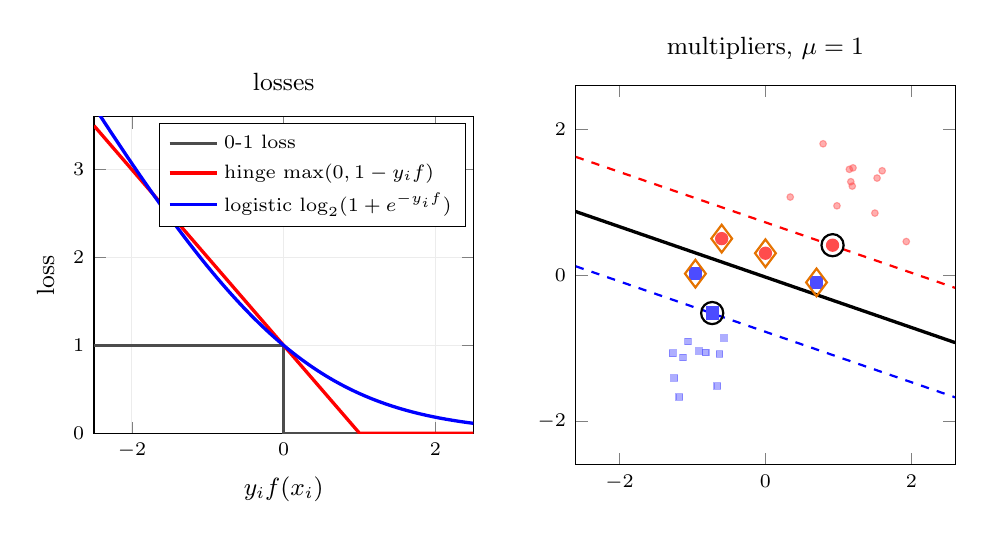
\begin{tikzpicture}
      \begin{axis}[name=loss, width=6.4cm, height=5.6cm, xmin=-2.5, xmax=2.5, ymin=0, ymax=3.6, xlabel={$y_if(\vect x_i)$}, ylabel={loss},
          title={losses}, title style={font=\small}, tick label style={font=\scriptsize}, label style={font=\small},
          legend style={font=\scriptsize, at={(0.98,0.98)}, anchor=north east}, legend cell align=left, grid=major, grid style={gray!15}]
        \addplot[gray!60!black, very thick, const plot] coordinates {(-2.5,1) (0,0) (2.5,0)};
        \addlegendentry{0-1 loss}
        \addplot[red, very thick, domain=-2.5:2.5, samples=81] {max(0,1-x)};
        \addlegendentry{hinge $\max(0,1-y_if)$}
        \addplot[blue, very thick, domain=-2.5:2.5, samples=81] {ln(1+exp(-x))/ln(2)};
        \addlegendentry{logistic $\log_2(1+e^{-y_if})$}
      \end{axis}
      \begin{axis}[at={(loss.east)}, anchor=west, xshift=1.3cm, width=6.4cm, height=6.4cm, axis equal image, xmin=-2.6, xmax=2.6, ymin=-2.6, ymax=2.6,
          xtick={-2,0,2}, ytick={-2,0,2}, tick label style={font=\scriptsize}, title={multipliers, $\mu=1$}, title style={font=\small}]
\addplot[only marks, mark=*, red!70, mark size=1.2pt, opacity=0.45, forget plot] coordinates {(1.20,1.47) (1.53,1.33) (1.93,0.46) (1.15,1.45) (1.19,1.22) (0.34,1.07) (0.79,1.80) (1.60,1.43) (1.17,1.28) (1.50,0.85) (0.98,0.95)};
\addplot[only marks, mark=square*, blue!70, mark size=1.2pt, opacity=0.45, forget plot] coordinates {(-1.27,-1.07) (-1.13,-1.13) (-0.66,-1.52) (-0.63,-1.08) (-1.25,-1.41) (-1.06,-0.91) (-0.91,-1.04) (-0.82,-1.06) (-0.57,-0.86) (-1.18,-1.67)};
\addplot[only marks, mark=*, red!70, mark size=2.2pt, forget plot] coordinates {(0.92,0.41)};
\addplot[only marks, mark=square*, blue!70, mark size=2.2pt, forget plot] coordinates {(-0.73,-0.52)};
\addplot[only marks, mark=o, mark size=4pt, thick, black, forget plot] coordinates {(0.92,0.41) (-0.73,-0.52)};
\addplot[only marks, mark=*, red!70, mark size=2.2pt, forget plot] coordinates {(0.00,0.30) (-0.60,0.50)};
\addplot[only marks, mark=square*, blue!70, mark size=2.2pt, forget plot] coordinates {(-0.96,0.02) (0.70,-0.10)};
\addplot[only marks, mark=diamond, mark size=5pt, thick, orange!90!black, forget plot] coordinates {(-0.96,0.02) (0.00,0.30) (-0.60,0.50) (0.70,-0.10)};
        \addplot[black, very thick] coordinates {(-2.600,0.871) (2.600,-0.925)};
        \addplot[red, dashed, thick] coordinates {(-2.600,1.621) (2.600,-0.175)};
        \addplot[blue, dashed, thick] coordinates {(-2.600,0.121) (2.600,-1.675)};
      \end{axis}
    \end{tikzpicture}
    \caption{Left: the hinge loss of the soft-margin SVM, $\xi_i=\max(0,1-y_if(\vect x_i))$, is a convex upper bound of the 0-1 loss. It is zero for samples beyond the margin ($y_if\ge1$) and grows linearly for margin violations; the logistic loss of logistic regression is a smooth alternative. Right: the soft-margin solution of Fig.~\ref{fig:svm_margin} with the Lagrange multipliers $\lambda_i$ from the dual problem. Faint samples: $\lambda_i=0$ (correct side of the margin, no influence on the solution). Black rings: $0<\lambda_i<\mu$ (exactly on a margin hyperplane, $\xi_i=0$). Orange diamonds: $\lambda_i=\mu$ (bounded support vectors, here margin violations with $\xi_i>0$). Only samples with $\lambda_i>0$ contribute to $\vect\alpha=\sum_i\lambda_iy_i\vect x_i$.}
    \label{fig:svm_losses}
  \end{figure}

  \textbf{Conclusion:} \\
 
  Feature vectors only appear in inner products, both in the learning and the classification phase.
  
\subsection{Feature Transforms}
 \textbf{Linear decision boundaries} in its current form have serious \textbf{limitations}:
  \begin{itemize}
    \item  Non-linearly separable data cannot be classified.
    \item  Noisy data cause problems. 
    \item  Formulation deals with vectorial data only.
  \end{itemize}
  \textbf{Possible solution:} 
  \begin{itemize}
    \item Map data into richer feature space using non-linear feature transform, \\
      then use a linear classifier.
  \end{itemize}
  We select a feature transform 
  \begin{displaymath}
    \phi: \real^d \rightarrow \real^D, \quad D \ge d
  \end{displaymath}
  such that the resulting features 
  \begin{displaymath}
    \phi(\vect x_i), \quad i = 1, 2, \dots, m
  \end{displaymath}
  are linearly separable.

    Example: Assume the decision boundary is given by the quadratic function
    \begin{displaymath}
      f(\vect x) = a_0 + a_1 x_1^2 + a_2 x_2^2 + a_3 x_1 x_2 + a_4 x_1+a_5 x_2.
    \end{displaymath}
    Obviously this is not a linear decision boundary. By the following mapping, we get features that have a linear decision boundary:
    \begin{displaymath}
      \phi(\vect x) = \left(\begin{array}{c}
                             1 \\ x_1^2 \\ x_2^2 \\ x_1x_2 \\ x_1 \\ x_2
                           \end{array}
                     \right)
    \end{displaymath}
  These feature transforms can be easily incorporated into SVMs:
  \begin{itemize}
    \item \textbf{Decision boundary:}
      {\small
        \begin{displaymath}
          f(\vect x) = \sum_i \lambda_i y_i \cdot  \langle\phi(\vect x_i), \phi(\vect x) \rangle + \alpha_0  
        \end{displaymath}
      }
      with predicted label $\hat y=\sign(f(\vect x))$ and decision boundary $\{\vect x: f(\vect x)=0\}$.
    \item The Lagrange dual problem is given by the \textbf{optimization problem}:
      {\small
        \begin{eqnarray*}
          \mbox{maximize} & -\frac{1}{2} \sum_i \sum_j \lambda_i \lambda_j y_i y_j \cdot \langle\phi(\vect x_i),\phi(\vect x_j)\rangle + \sum_i \lambda_i \\   
          \mbox{subject to}  & \vect{\lambda}\succeq 0, \quad \sum_{i} \lambda_i \, y_i = 0
        \end{eqnarray*}
      }
      (hard margin; for the soft margin add $\lambda_i\le\mu$).
  \end{itemize}
 
\subsection{Kernel Functions}

  We now define \textbf{kernel functions}:
  \begin{displaymath}
    k(\vect x, \vect x') =  \langle \phi(\vect x), \phi(\vect x') \rangle
  \end{displaymath}
  Typical kernel functions are:
  \begin{itemize}
    \item \textbf{Linear:} 
      \begin{displaymath}
        k(\vect x, \vect x') =~ \langle\vect x, \vect x'\rangle
      \end{displaymath}
    \item \textbf{Polynomial:} 
      \begin{displaymath}
        k(\vect x, \vect x') = (\langle\vect x, \vect x'\rangle + 1)^q, \quad q\in\mathbb N
      \end{displaymath}
    \item \textbf{Radial basis function:} 
      \begin{displaymath}
        k(\vect x, \vect x') = e^{-\gamma\|\vect x- \vect x'\|_2^2}
      \end{displaymath}
    \item \textbf{Sigmoid kernel:} 
      \begin{displaymath}
        k(\vect x, \vect x') =\mbox{tanh}({ \kappa \langle\vect x, \vect x'\rangle + c}), \quad \kappa>0
      \end{displaymath}
      (not positive semidefinite for all $\kappa, c$, so strictly not always a valid kernel; see Chapter \emph{Kernels})
  \end{itemize}
  
\subsection{Lessons Learned}

  \begin{itemize}
    \item Lagrangian formulation of the hard and soft margin problems    
    \item Lagrange dual representation    
    \item Idea of feature transforms
  \end{itemize}

\subsection{Comprehensive Questions}

  \begin{itemize}
    \item What is the Lagrangian of the hard margin SVM? 
    \item What are the KKT optimality conditions for the hard margin SVM? 
    \item How do we apply the KKT conditions to the Lagrange Dual? 
    \item What can we conclude from this reformulated Lagrange Dual?
  \end{itemize}
  

